%%% demothesis.tex --- 
%% 
%% Filename: demothesis.tex
%% Description: 
%% Author: Ola Leifler
%% Maintainer: 
%% Created: Thu Oct 14 12:52:20 2010 (CEST)
%% Version: $Id$
%% Version: 
%% Last-Updated: Wed Jun 28 10:57:24 2017 (+0200)
%%           By: Ola Leifler
%%     Update #: 169
%% URL: 
%% Keywords: 
%% Compatibility: 
%% 
%%%%%%%%%%%%%%%%%%%%%%%%%%%%%%%%%%%%%%%%%%%%%%%%%%%%%%%%%%%%%%%%%%%%%%
%% 
%%% Commentary: 
%% 
%% 
%% 
%%%%%%%%%%%%%%%%%%%%%%%%%%%%%%%%%%%%%%%%%%%%%%%%%%%%%%%%%%%%%%%%%%%%%%
%% 
%%% Change log:
%% 
%% 
%% RCS $Log$
%%%%%%%%%%%%%%%%%%%%%%%%%%%%%%%%%%%%%%%%%%%%%%%%%%%%%%%%%%%%%%%%%%%%%%
%% 
%%% Code:

% !TeX program = xelatex

\documentclass[msc, filfak, english]{liuthesis}
%% Settings go in settings.tex
%%% settings.tex --- 
%% 
%% Filename: settings.tex
%% Description: 
%% Author: Ola Leifler
%% Maintainer: 
%% Created: Tue Oct 19 21:11:31 2010 (CEST)
%% Version: $Id$
%% Version: 
%% Last-Updated: Tue Apr 25 08:49:48 2017 (+0200)
%%           By: Ola Leifler
%%     Update #: 43
%% URL: 
%% Keywords: 
%% Compatibility: 
%% 
%%%%%%%%%%%%%%%%%%%%%%%%%%%%%%%%%%%%%%%%%%%%%%%%%%%%%%%%%%%%%%%%%%%%%%
%% 
%%% Commentary: 
%% 
%% 
%% 
%%%%%%%%%%%%%%%%%%%%%%%%%%%%%%%%%%%%%%%%%%%%%%%%%%%%%%%%%%%%%%%%%%%%%%
%% 
%%% Change log:
%% 
%% 
%% RCS $Log$
%%%%%%%%%%%%%%%%%%%%%%%%%%%%%%%%%%%%%%%%%%%%%%%%%%%%%%%%%%%%%%%%%%%%%%
%% 
%%% Code:

\usepackage[ruled,vlined]{algorithm2e}

\usepackage[backend=biber,hyperref, style =authoryear]{biblatex}
%\nocite{*}
%% To set the font of your thesis, use the \setmainfont{} command,
%% surrounded with \ifxetex if you want to switch between xelatex and pdflatex
\ifxetex 
%\setmainfont [Scale=1]{Calibri}
\fi

%%%%%%%%%%%%
%% The VZ43 chapter style, from Memoir contributed chapter styles: ftp://ftp.tex.ac.uk/ctan%3A/info/MemoirChapStyles/MemoirChapStyles.pdf
%%%%%%%%%%%

\usepackage{calc,color}
\newif\ifNoChapNumber
\newcommand\Vlines{%
\def\VL{\rule[-2cm]{1pt}{5cm}\hspace{1mm}\relax}
\VL\VL\VL\VL\VL\VL\VL}
\makeatletter
\setlength\midchapskip{0pt}
\makechapterstyle{VZ43}{
\renewcommand\chapternamenum{}
\renewcommand\printchaptername{}
\renewcommand\printchapternum{}

\renewcommand\chapnumfont{\Huge\bfseries\centering}
\renewcommand\chaptitlefont{\Huge\bfseries\raggedright}
\renewcommand\printchaptertitle[1]{%
\Vlines\hspace*{-2em}%
\begin{tabular}{@{}p{1cm} p{\textwidth-3cm}}%
\ifNoChapNumber\relax\else%
\colorbox{black}{\color{white}%
\makebox[.8cm]{\chapnumfont\strut \thechapter}}
\fi
& \chaptitlefont ##1
\end{tabular}
\NoChapNumberfalse
}
\renewcommand\printchapternonum{\NoChapNumbertrue}
}
\makeatother


%% To set bibliography options, refer to the biblatex manual and use
%% the ExecuteBibliographyOptions command below to set your options

\ExecuteBibliographyOptions{maxnames=99}


%% Change this to your appropriate BibTeX reference file (.bib)

\addbibresource{references.bib}

%%%%%%%%%%%%%%%%%%%%%%%%%%%%%%%%%%%%%%%%%%%%%%%%%%%%%%%%%%%%%%%%%%%%%%
%%% settings.tex ends here

%%% Local Variables: 
%%% mode: latex
%%% TeX-master: "demothesis"
%%% End: 

\usepackage{rotating}
\usepackage{color}

\usepackage[acronym, toc]{glossaries}
\makenoidxglossaries

\newacronym{gbco}{GBCO}{Gate Bias Cycled Operation}

\newacronym{tco}{TCO}{Temperature Cycled Operation}

\newacronym{sicfet}{SiC-FET}{Silicon Carbide Field Effect Transistor}

\newacronym{scr}{SCR}{Selective Catalytic Reduction}

\newacronym{plsr}{PLSR}{Partial Least Squares Regression}


\usepackage{hyphenat}
\setlength{\parskip}{0.8em}

%% Handling NOX and chemical formulas{\tiny }
\usepackage{chemformula}
\usepackage{xspace}
\usepackage{fixltx2e}
\usepackage{subscript}
\newcommand{\nox}{\texorpdfstring{NO\textsubscript{x}}{NOx}\xspace}
%%

\department{Institutionen för datavetenskap}
\departmentenglish{Department of Computer and Information Science}
\departmentshort{IDA}
% If this is a thesis at the cognitive science study programme, use
% the "area" command to generate a proper (?) ISRN
% \area{KOGVET-A}

% Include an external supervisor on the cover page
% \externalsupervisor{Min företagshandledare}
\externalsupervisor{Mike Andersson}
\supervisor{Annika Tillander}

\examiner{José M. Peña}
\titleenglish{\nohyphens{Quantifying nitrogen oxides and ammonia via frequency modulation in gas sensors}}
\subtitleenglish{\textcolor{red}{\textbf{DRAFT}}}
\titleswedish{Kvantifiering av kväveoxider och ammoniak via frekvensmodulering i gassensorer}
\thesissubject{Statistics and Machine Learning}

\publicationyear{2021}
\currentyearthesisnumber{001}
\dateofpublication{2021-MM-DD}

\author{Marcos Freitas Mourão dos Santos}

\usepackage{setspace}
\linespread{1.3}

\setcounter{secnumdepth}{3}
\DeclareMathOperator{\Tr}{Tr}
\begin{document}
\chapterstyle{VZ43}

% List of acronyms
%\printnoidxglossary[type=acronym]


%%% Intro.tex --- 
%% 
%% Filename: Intro.tex
%% Description: 
%% Author: Ola Leifler
%% Maintainer: 
%% Created: Thu Oct 14 12:54:47 2010 (CEST)
%% Version: $Id$
%% Version: 
%% Last-Updated: Thu May 19 14:12:31 2016 (+0200)
%%           By: Ola Leifler
%%     Update #: 5
%% URL: 
%% Keywords: 
%% Compatibility: 
%% 
%%%%%%%%%%%%%%%%%%%%%%%%%%%%%%%%%%%%%%%%%%%%%%%%%%%%%%%%%%%%%%%%%%%%%%
%% 
%%% Commentary: 
%% 
%% 
%% 
%%%%%%%%%%%%%%%%%%%%%%%%%%%%%%%%%%%%%%%%%%%%%%%%%%%%%%%%%%%%%%%%%%%%%%
%% 
%%% Change log:
%% 
%% 
%% RCS $Log$
%%%%%%%%%%%%%%%%%%%%%%%%%%%%%%%%%%%%%%%%%%%%%%%%%%%%%%%%%%%%%%%%%%%%%%s
%% 
%%% Code:

\chapter{Introduction}
\label{cha:introduction}

\section{Motivation}
\label{sec:motivation}

Nitric Oxide ({\ch{NO}) and Nitrogen Dioxide (\ch{NO2}), commonly referred together as \nox,  are hazardous gases to the environment and to humans. Its main sources are combustion processes in transportation, and industrial processes such as (but not limited to) automobiles, trucks, boats, industrial boilers, turbines, etc. \parencite{EPA_2019}.

\nox exposure to humans can cause respiratory illnesses such as bronchitis, emphysema and can worsen heart disease \parencite{Boningari_2016}. Environmentally, \nox are deemed precursors of adverse phenomena such as smog, acid rain, and the depletion of ozone (\ch{O3}) \parencite{Bernabeo_2019}. It is of high interest, therefore, to reduce \nox emissions.

One well studied and successful method of reducing emissions is \acrfull{scr}, which consists of the reduction of \nox by ammonia (\ch{NH3}) into nitrogen gas (\ch{N2}) and water (\ch{H2O}) \parencite{Forzatti_2001}, both harmless components. The process is based on the following reactions \parencite{Forzatti_2001}:
\begin{itemize}
	\item \ch{4 NH3 + 4 NO + O2 -> 4 N2 + 6 H2O}
	
	\item \ch{2 NH3 + NO + NO2 -> 2 N2 + 3 H2O}
	
	\item \ch{8 NH3 + 6 NO2 -> 7 N2 + 12 H2O}
\end{itemize}


One key element in these reactions, however, is the amount of ammonia dosed into the \acrshort{scr} systems. Ammonia itself is hazardous to humans, causing skin and respiratory irritation, among other illnesses \parencite{ASTDRA_2004}. More importantly, ammonia is one of the main sources of nitrogen pollution, and it has a direct negative impact on biodiversity via nitrogen deposition in soil and water \parencite{RAND_2018}. Hence it is also desired to keep ammonia emissions to a minimum. Too much ammonia in the \acrshort{scr} catalyst will guarantee \nox reduction at the expense of undesired ammonia emissions. Concurrently, too little ammonia will impede \acrshort{scr} from occurring properly, beating the purpose of the catalyst and consequently, there will be undesired \nox emissions.

To monitor gases concentrations, chemical sensors are deployed, one of which is the \acrfull{sicfet}. The identification and quantification of gases is normally achieved through multiple sensors in so-called sensor arrays. Ideally, each sensor in the array needs to have different responses to different compounds \parencite{Bastuck_2019}. The deployment of multiple sensors, on the other hand, proves itself cumbersome due to the increased chances of failure and decalibration of the system should one or multiple sensors be replaced \parencite{Bastuck_2019}.

One solution to this problem is the cycled operation of one single sensor, referred as a virtual multi-sensor \parencite{Bastuck_2019}. By cycling the working point parameters of the sensor, different substances react differently in the sensor surface, which in turn produces different responses. \acrfull{tco}, \acrfull{gbco}, and the combination of the two have been proven to increase the selectivity of \acrshort{sicfet} sensors \parencite{Bastuck_2019}.

\acrshort{tco}, in contrast with a constant temperature evaluation, produces unique transient sensor responses, i.e. each gas mixture yields a slightly different sensor output. This unique gas signature increases selectivity \parencite{bur2014}. Additionally, the high temperatures reached in these cycles help in the cleansing of the sensor surface, preparing it for the new mixtures to come.

Frequency modulation tries to achieve the same goal: avoid steady-state responses in exchange of unique signatures that could help identify/quantify the gases at hand. It consists on operating the sensor in \acrfull{ac}. One then can regulate the frequency of this operation and create cycles of different frequencies, similar to what is done in \acrshort{tco}. This is somewhat similar to \acrshort{gbco} but with more frequency changes and achieving overall higher frequencies. For this reason, investigation of this new technique is of interest.

\section{Aim}
\label{sec:aim}

The aim of this thesis is to investigate if frequency modulation can be used to simultaneously quantify the concentrations of \nox and Ammonia in a particular gas mixture. Frequency modulation, as described above, was not used beforehand

\section{Research questions}
\label{sec:research-questions}

\begin{enumerate}
	\item Can frequency modulation be used to simultaneously quantify \nox and Ammonia concentrations?
	%\item Is it possible to achieve acceptable prediction levels for \nox and Ammonia using frequency modulation?
	\item Does the quality of fit vary over different prediction models?
\end{enumerate}

%\nocite{scigen}
%We have included Paper \ref{art:scigen}

%%%%%%%%%%%%%%%%%%%%%%%%%%%%%%%%%%%%%%%%%%%%%%%%%%%%%%%%%%%%%%%%%%%%%%
%%% Intro.tex ends here


%%% Local Variables: 
%%% mode: latex
%%% TeX-master: "demothesis"
%%% End: 

\chapter{Data}
\label{cha:data}

\section{Data acquisition}
\label{sec:data-acquisition}

The data was acquired at the \acrfull{sas} laboratory at Linköping University. The experiment --- as shown in Figure~\ref{fig:experimental-setup} --- consisted of exposing different gas combinations to two \acrshort{sicfet} sensors under a particular frequency cycle and recording its response, measured in \acrfull{ma}. The response is then used to extract secondary features, namely average and slope values from certain regions of the frequency cycle. These shape-defining features were not chosen randomly; they are staples in the literature and are promising to this type of problem \parencite{Bastuck_2019} \parencite{Bur791934}.

\begin{figure}[!htb]
	\centering
	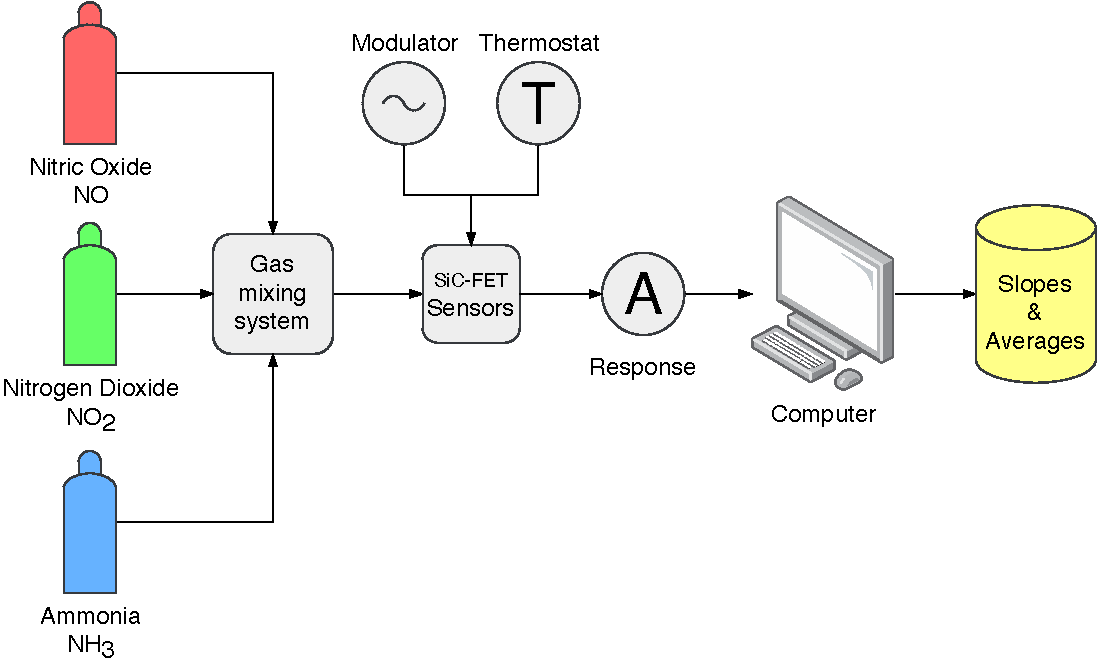
\includegraphics[width=0.8\textwidth]{../figures/experimental-setup.pdf}
	\caption{Schema of the data acquisition process.}
	\label{fig:experimental-setup}
\end{figure}

In more detail, \ch{NO}, \ch{NO2} and \ch{NH3} had five possible concentration values each: 5, 10, 20, 40, and 80 \acrfull{ppm}. The experiment was designed to encompass all possible combinations of these gases, amounting to 125 different gas mixtures. Each feature was submitted to the same frequency cycle four times. The cycle consists of 16 unique frequencies: 0.05, 0.1, 0.25, 0.5, 1, 2, 5, 10, 25, 50, 100, 200, 500, 1000, 2500 and 5000 \acrfull{hertz}. A typical raw sensor response for frequency modulation experiments is shown in Figure~\ref{fig:raw}.

\begin{figure}[!htb]
	\centering
	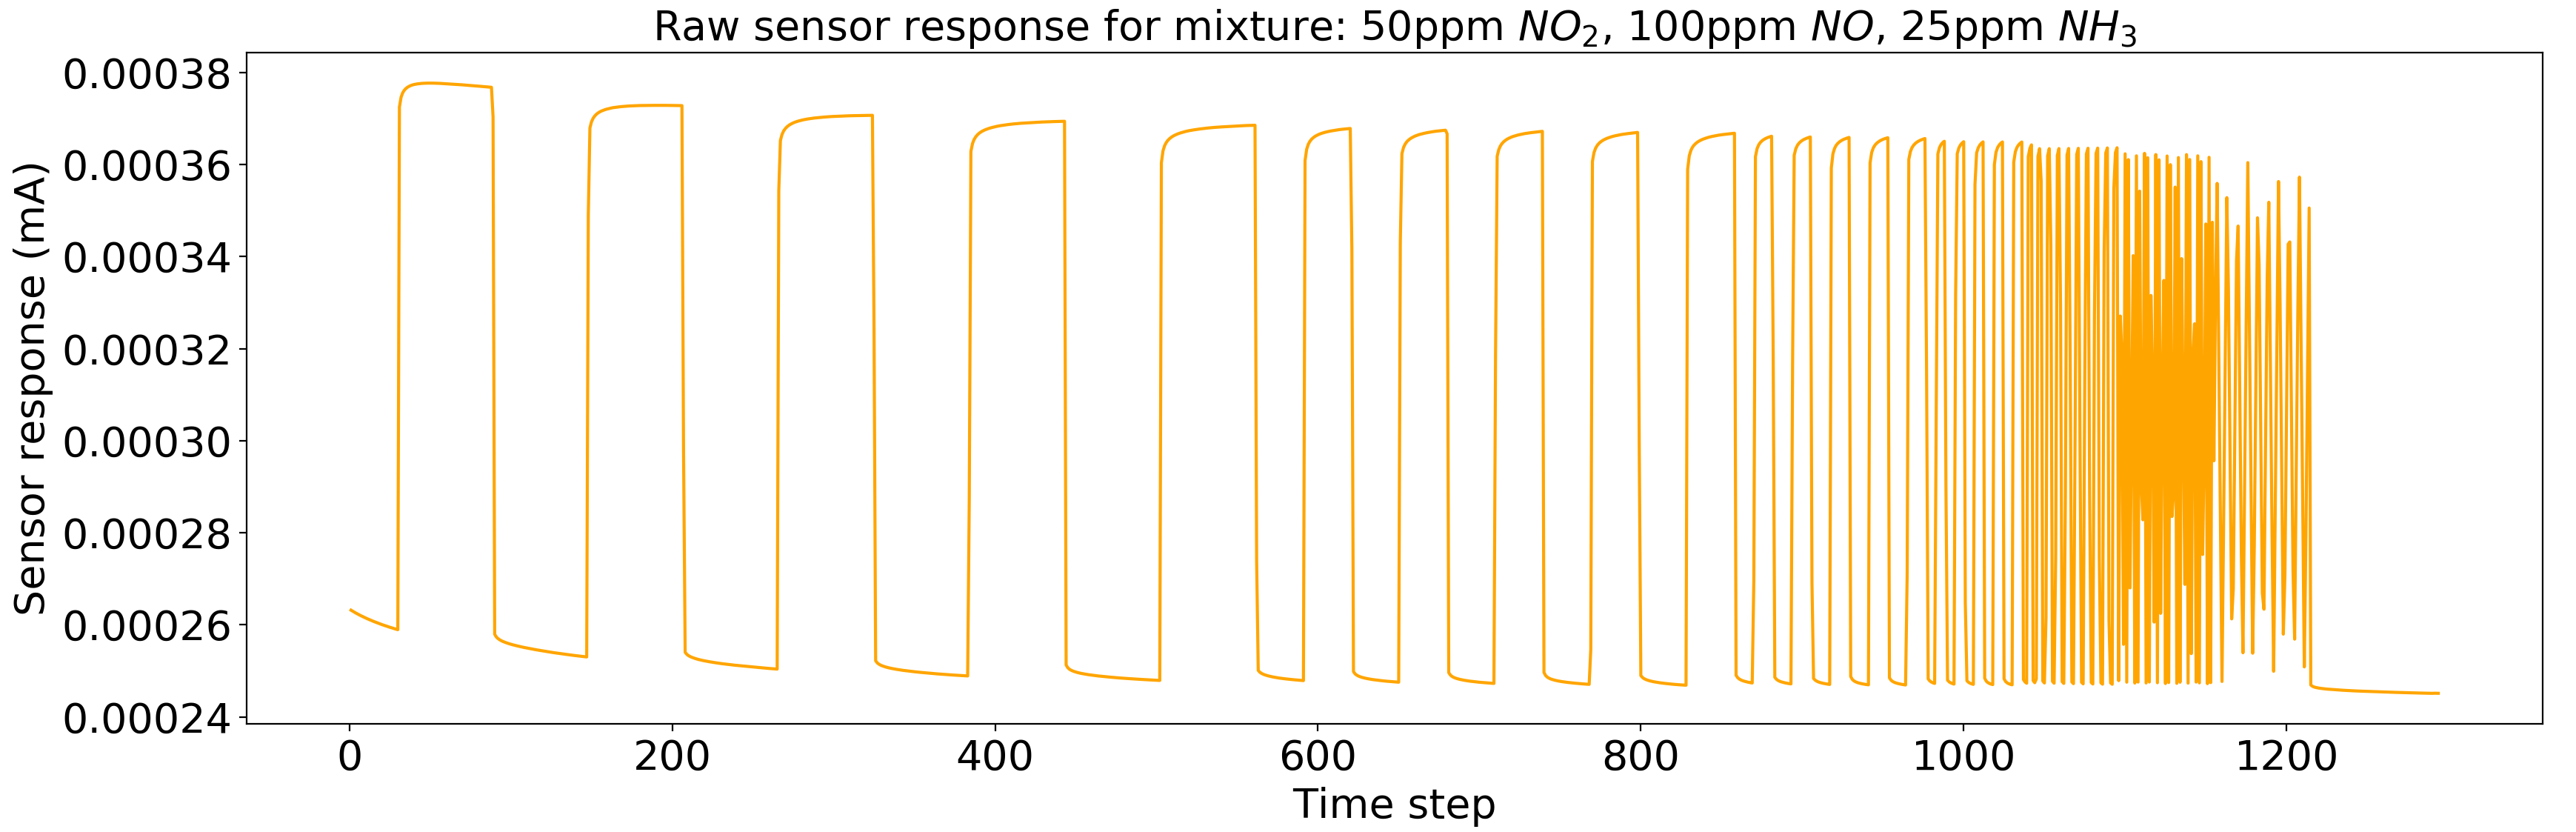
\includegraphics[width=1\textwidth]{../figures/raw-response.png}
	\caption{An example of raw sensor response}
	\label{fig:raw}
\end{figure}

Throughout one cycle, several slope and average features were extracted. The sample rate for feature extraction was set at 4 \acrshort{hertz}, i.e. in a cycle of 60 seconds, a total of $60 \text{s} \times 4 \frac{1}{\text{s}} = 240$ pairs of slopes and averages are recorded, which totals to 480 features per cycle. In other words, during one experiment --  4 cycles of 60 seconds -- a total of $480 \times 4 = 1920$ features are extracted. 

One way to visualize the above process is shown in Figures~\ref{fig:feat-window}. Note that the y-axis is in log-scale due to the different orders of magnitude of frequencies. Moreover, Figure~\ref{fig:features} gives more insight into feature measurement, and Table~\ref{tab:measurements} summarizes the data acquisition details.

\begin{figure}[!htb]
	\centering
	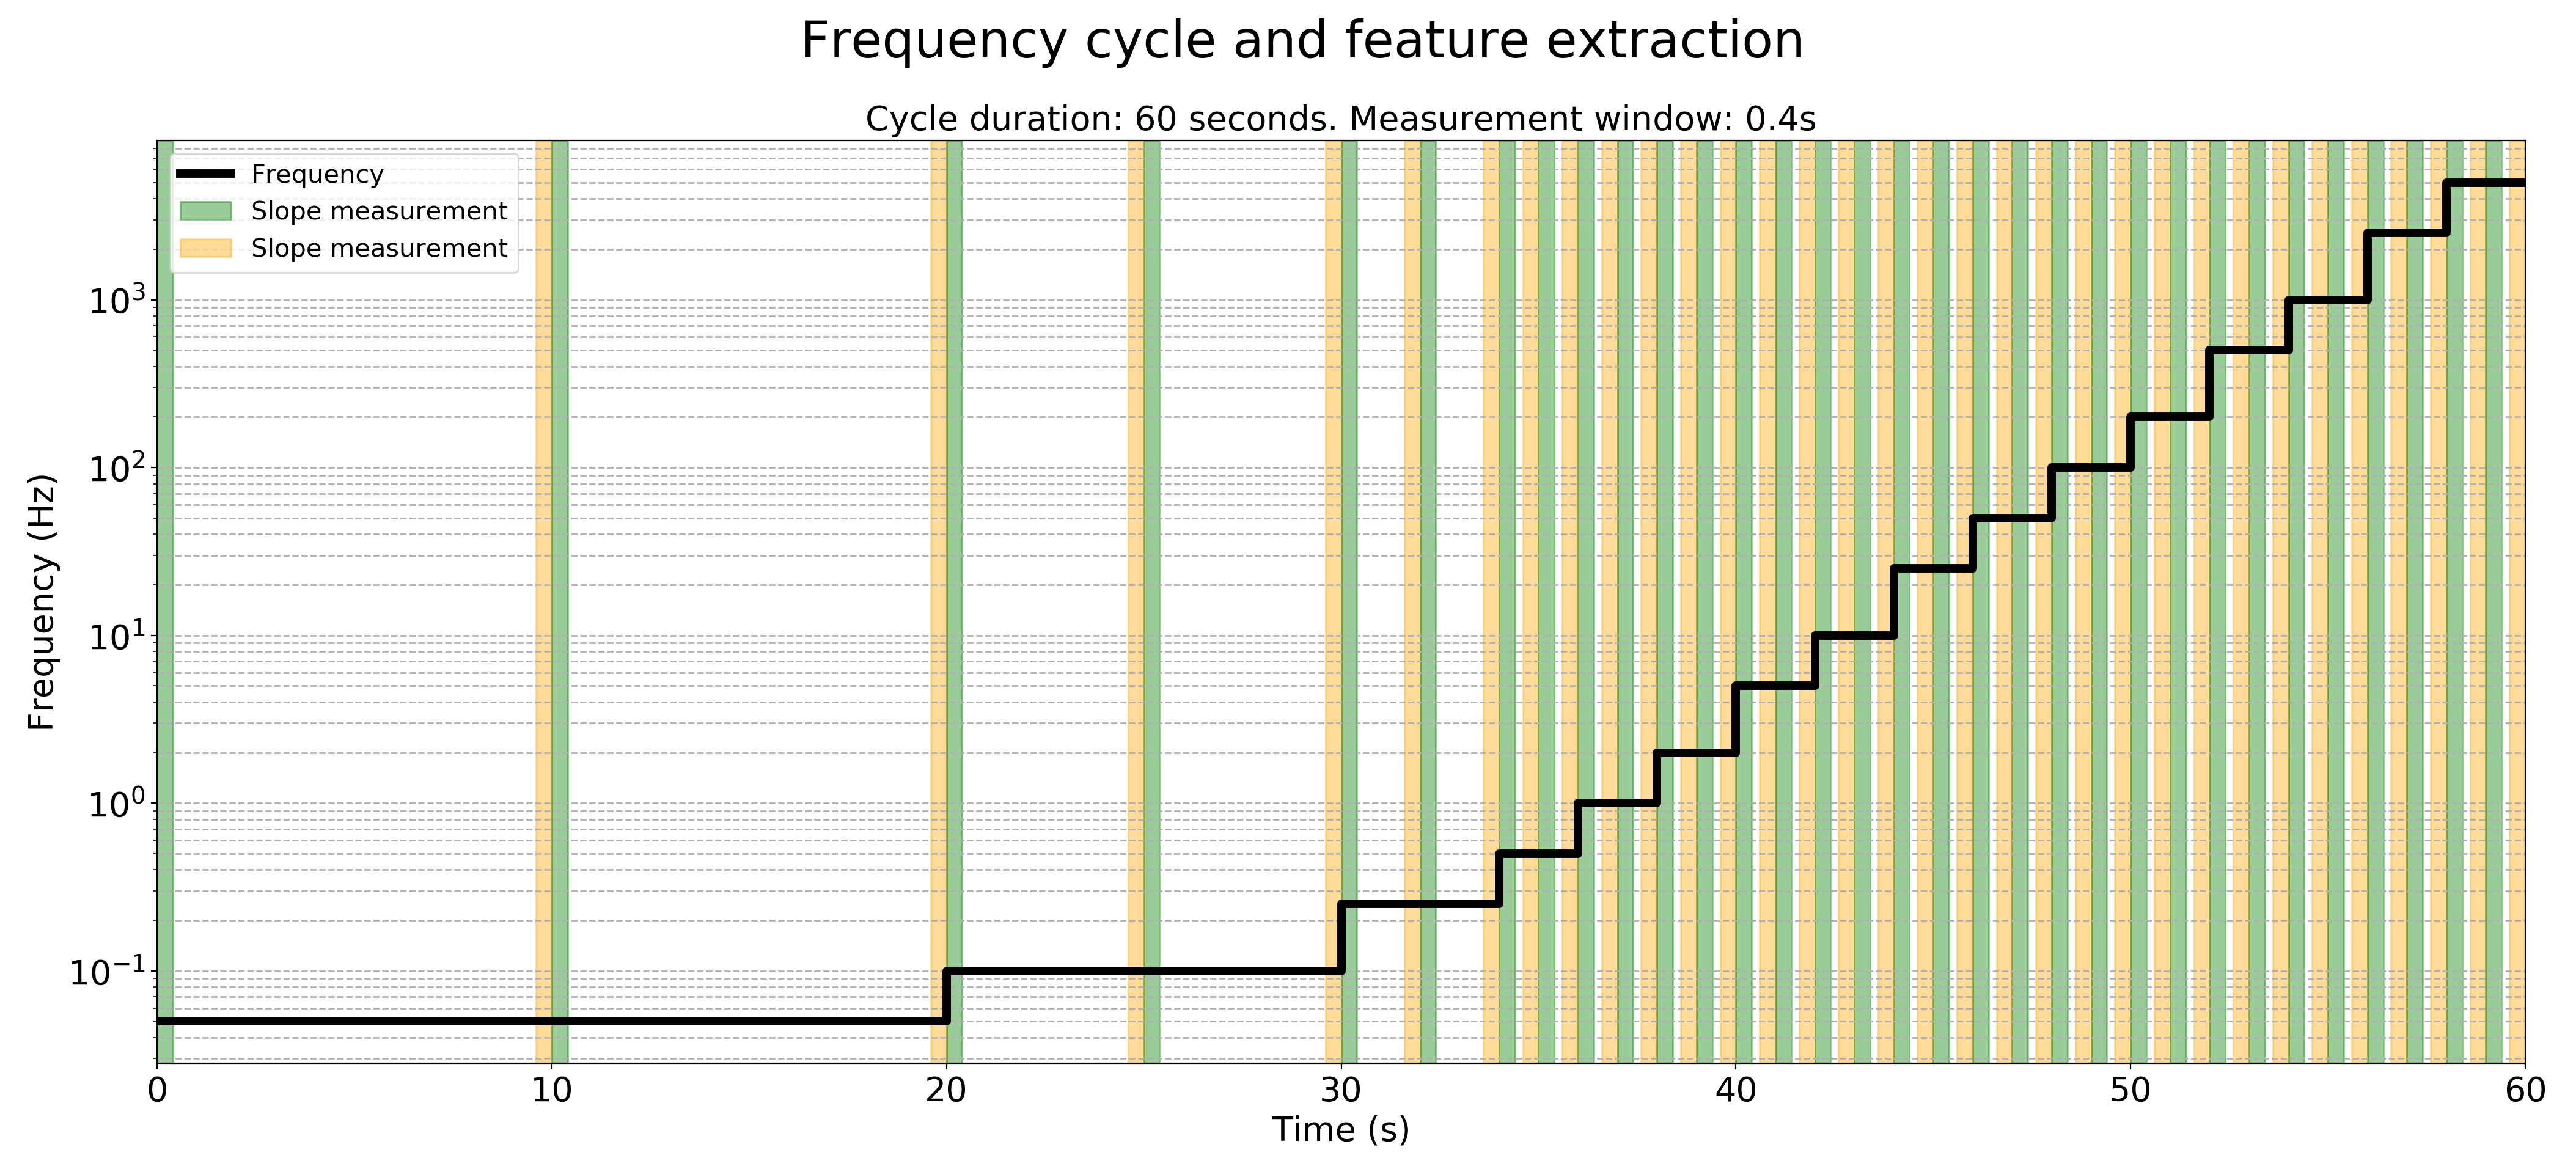
\includegraphics[width=0.9\textwidth]{../figures/measurement-windows.png}
	
	\caption{Feature measurements times per cycle. The width of the red line indicates the duration of one of the feature measurement windows as an example.}
	\label{fig:feat-window}
\end{figure} 

\begin{figure}[h]
	\centering
	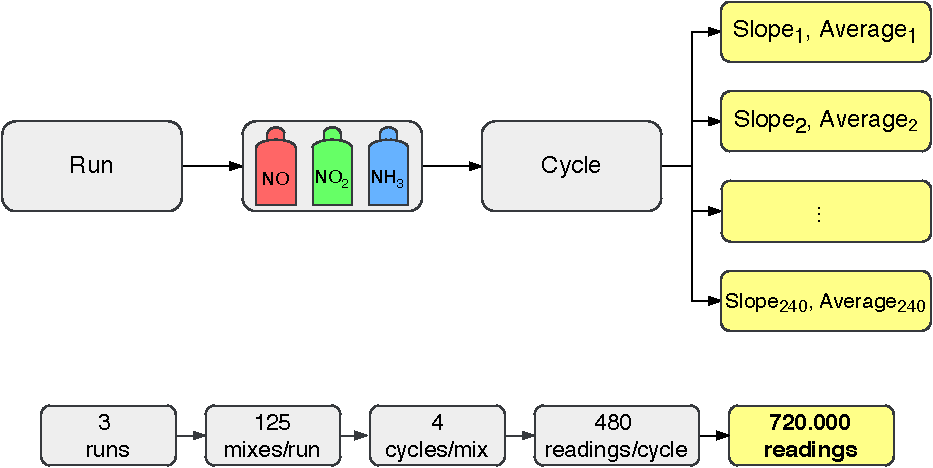
\includegraphics[width=0.9\textwidth]{../figures/features.pdf}
	\caption{A visualization of the feature measurement process.}
	\label{fig:features}
\end{figure}

\begin{table}[h]
	\centering
	\caption{Data acquisition details}
	\label{tab:measurements}
	\begin{tabular}{|c|c|}
		\hline
		\textbf{Parameter} & \textbf{Value} \\
		\hline
		Factors (gases) & 3 \\
		\hline
		Levels (concentrations) & 5 \\
		\hline
		Frequencies & 16 \\
		\hline
		Features per cycle & 480 \\
		\hline
		Number of cycles & 4 \\
		\hline
		Data points per mixture & 1920\\
		\hline
		Number of mixtures & 125 \\
		\hline
		Features per experiment & 240.000 \\
		\hline
		Number of experiments & 3 \\
		\hline
		Total features & 720.000 \\
		\hline
	\end{tabular}
\end{table}

For specific timestamps and measurement durations, the reader is referred to Appendix~\ref{app:A}.

\section{Raw data}
\label{sec:raw-data}

The experiments were run between 26th and 29th March 2021. The experiment data was exported as an excel file containing twelve columns, as specified in Table~\ref{tab:raw-cols}


\begin{table}[h]
	\centering
	\caption{Raw data column details}
	\label{tab:raw-cols}
	
	\resizebox{\textwidth}{!}{%
		\begin{tabular}{|c|c|c|}
		\hline
		\textbf{Name} & \textbf{Description} & \textbf{Unit} \\
		\hline
		Exposure nr & A particular mix of NO, NO$_2$ and NH$_3$. Ranges from 1 to 375  & -\\
		\hline
		Cycle nr & The cycle number. Ranges from 1 to 4. & - \\
		\hline
		Sample nr & Extracted feature index. Ranges from 1 to 240 & - \\
		\hline
		NO & Nitric Oxide concentration & \acrshort{ppm} \\
		\hline
		NO2 & Nitrogen Dioxide concentration &\acrshort{ppm} \\
		\hline
		NH3 & Ammonia concentration &\acrshort{ppm} \\
		\hline
		Freq & Frequency & \acrshort{hertz}\\
		\hline
		Slope sensor 1 & Slope & $\mu$A/s \\
		\hline
		Slope sensor 2 & Slope & $\mu$A/s\\
		\hline
		Average sensor 1 & Average & $\mu$A \\
		\hline
		Average sensor 2& Average & $\mu$A\\
		\hline
		Sensor temperature & Temperature & degrees Celsius ($^{\circ}$C) \\
		\hline
	\end{tabular}}
\end{table}

\begin{table}
	\centering
	\caption{Sample of raw data.}
	\label{tab:raw-sample}
	\resizebox{\textwidth}{!}{%
		\begin{tabular}{p{1.5cm}p{1.3cm}p{0.8cm}p{1.3cm}p{0.8cm}p{0.8cm}p{1.8cm}p{1.8cm}p{1.8cm}p{1.8cm}p{1.8cm}p{1.8cm}p{1.8cm}}
		\toprule[0.5mm]
		Index & Exposure\newline nr &  Cycle\newline  nr &  Sample\newline  nr &  NO\newline  [ppm] &  NO2\newline  [ppm] &  NH3\newline  [ppm] &  Freq\newline  [Hz] &  Slope\newline  sensor 1\newline [$\mu$A/s] &  Slope\newline  sensor 2\newline [$\mu$A/s] &  Average\newline  sensor 1\newline [$\mu$A] &  Average\newline  sensor 2\newline [$\mu$A] &  Sensor\newline  temperature \newline[C] \\
		\midrule[0.5mm]
		0 &            1 &         1 &          1 &        10 &          5 &         20 &       0.05 &             -18.855169 &             -22.588416 &                32.926184 &                27.961554 &              274.994683 \\
		1 &            1 &         1 &          2 &        10 &          5 &         20 &       0.05 &             -28.289268 &             -28.185027 &                25.853867 &                20.915297 &              274.980487 \\
		2 &            1 &         1 &          3 &        10 &          5 &         20 &       0.05 &              -0.390916 &              -0.482129 &                25.756138 &                20.794765 &              274.985895 \\
		3 &            1 &         1 &          4 &        10 &          5 &         20 &       0.05 &              -0.234549 &              -0.156366 &                25.697501 &                20.755673 &              275.020372 \\
		4 &            1 &         1 &          5 &        10 &          5 &         20 &       0.05 &              -0.143336 &              -0.247580 &                25.661667 &                20.693778 &              275.014964 \\
		
		\bottomrule
		&&&&&&&&&&&&\\
		&&&&&&&\sbox0{\dots}\makebox[\wd0]{\vdots}&&&&&\\
		&&&&&&&&&&&&\\
		\toprule
		
		100000 &          105 &         1 &        161 &         5 &          5 &         40 &        5.0 &             -38.366212 &             -48.495271 &                30.241896 &                24.821197 &              275.021724 \\
		100001 &          105 &         1 &        162 &         5 &          5 &         40 &        5.0 &               6.619507 &               8.521964 &                31.896773 &                26.951688 &              274.999415 \\
		100002 &          105 &         1 &        163 &         5 &          5 &         40 &        5.0 &              -1.941549 &               6.580416 &                31.411386 &                28.596792 &              275.011584 \\
		100003 &          105 &         1 &        164 &         5 &          5 &         40 &        5.0 &              27.401023 &              22.012900 &                38.261641 &                34.100017 &              275.009894 \\
		100004 &          105 &         1 &        165 &         5 &          5 &         40 &        5.0 &             -27.016623 &             -28.439121 &                31.507486 &                26.990236 &              275.014400 \\
		\bottomrule
		&&&&&&&&&&&&\\
		&&&&&&&\sbox0{\dots}\makebox[\wd0]{\vdots}&&&&&\\
		&&&&&&&&&&&&\\
		\toprule
		
		359995 &          375 &         4 &        236 &        20 &         80 &          5 &     5000.0 &              -0.136821 &              -0.158538 &                34.129879 &                30.345597 &              275.002007 \\
		359996 &          375 &         4 &        237 &        20 &         80 &          5 &     5000.0 &               0.010859 &               0.010859 &                34.132593 &                30.348312 &              274.986797 \\
		359997 &          375 &         4 &        238 &        20 &         80 &          5 &     5000.0 &              -0.043435 &               0.030405 &                34.121734 &                30.355913 &              274.979811 \\
		359998 &          375 &         4 &        239 &        20 &         80 &          5 &     5000.0 &              -0.117275 &              -0.026061 &                34.092416 &                30.349398 &              274.984543 \\
		359999 &          375 &         4 &        240 &        20 &         80 &          5 &     5000.0 &               0.073840 &               0.039092 &                34.110876 &                30.359171 &              274.998063 \\
		\bottomrule[0.5mm]
	\end{tabular}}
\end{table}

\newpage
\section{Pre-processing}
\label{sec:preprocessing}

The features (slopes and averages) from the same target (a particular exposure) in the raw data file in Table~\ref{tab:raw-sample} are spread across multiple rows, which is not suitable for analysis, as different features from the same observation as spread along multiple columns. As opposed to \acrshort{tco}, the experiments were conducted at constant temperature, and therefore, the temperature column is discarded. The data was, subsequently, modified to have the desired format: each row containing the predictors for one particular combination of gases. Additionally, the data from each sensor was split into  two datasets. 

The naming convention for the features is shown in Figure~\ref{fig:feat-naming}. First, the frequency in which the measurement was taken followed by the sensor number. After that, the feature name itself is followed by its index, i.e. where in the frequency cycle the measurement was made. This convention allows for easy identification of key information of the cycle and measurement.

\begin{figure}[h]
	\centering
	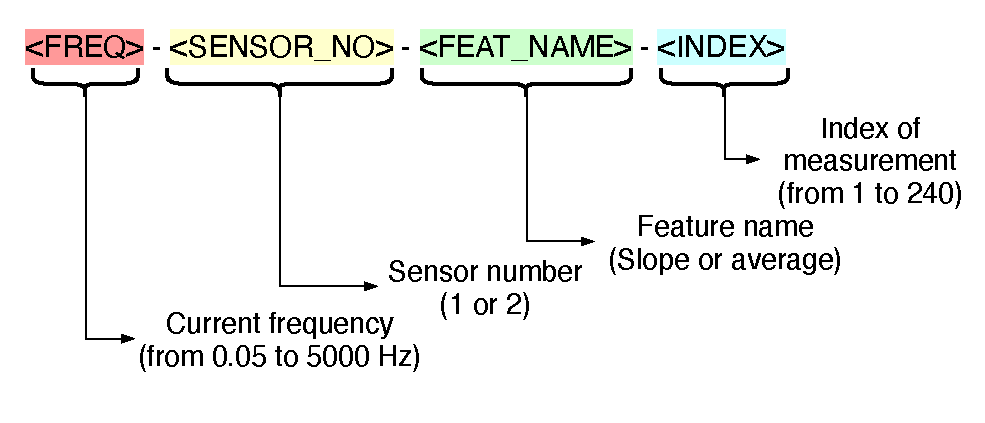
\includegraphics[width=1\textwidth]{../figures/feat-naming.pdf}
	\caption{Feature naming convention.}
	\label{fig:feat-naming}
\end{figure}

The pre-processing results in the format shown in Figure~\ref{fig:preprocessed-data}. Recalling that there are 125 possible mixtures of gases, it is important to note that there are repeated exposures in the data set, and those are treated as individual observations. Since each unique gas mixture was exposed 4 times during a cycle, and the experiment was repeated 3 times, this yields a total of $4 \times 3 \times 125 = 1500$ exposures. A snippet of the final data set is shown in Table~\ref{tab:prepro-sample}.

\begin{figure}[h]
	\centering
	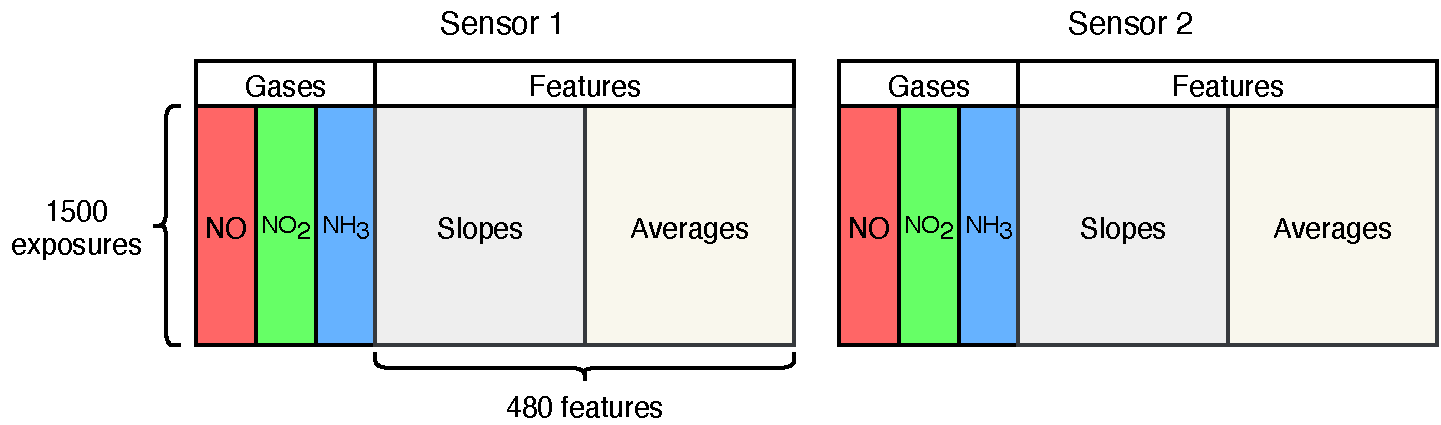
\includegraphics[width=1\textwidth]{../figures/preprocessed-data.pdf}
	\caption{Pre-processed data structure.}
	\label{fig:preprocessed-data}
\end{figure}

\begin{table}
	\centering
	\caption{Sample of pre-processed data.}
	\label{tab:prepro-sample}
	\resizebox{\textwidth}{!}{%
	\begin{tabular}{ccp{0.8cm}p{0.8cm}p{0.8cm}p{1.8cm}p{1.8cm}p{0.3cm}p{1.6cm}p{1.6cm}p{1.6cm}p{1.6cm}p{0.3cm}p{1.6cm}p{1.6cm}}
		\toprule[0.5mm]
		Index &  EXPOSURE &    NO &   NO2 &   NH3 &  0.05-1-slope-0 &  0.05-1-slope-1 & $\dots$&  5000.0-1-slope-239 &  0.05-1-avg-0 &  0.05-1-avg-1 &  0.05-1-avg-2 & $\dots$&  5000.0-1-avg-238 &  5000.0-1-avg-239 \\
		\midrule[0.5mm]
		0 &       1.0 &  10.0 &   5.0 &  20.0 &      -18.855169 &      -28.289268 &$\dots$&            0.019546 &     32.926184 &     25.853867 &     25.756138 &$\dots$&         35.840135 &         35.845021 \\
		1 &       1.0 &  10.0 &   5.0 &  20.0 &      -28.979886 &       -9.251672 &$\dots$&           -0.056466 &     28.600050 &     26.287132 &     26.225237 & $\dots$&        35.884113 &         35.869996 \\
		2 &       1.0 &  10.0 &   5.0 &  20.0 &      -25.431240 &      -12.874158 &$\dots$&           -0.052122 &     29.512187 &     26.293647 &     26.238267 & $\dots$&        35.913432 &         35.900401 \\
		3 &       1.0 &  10.0 &   5.0 &  20.0 &      -30.126572 &       -8.196200 &$\dots$&           -0.156366 &     28.368758 &     26.319708 &     26.254555 &$\dots$&         35.939493 &         35.900401 \\
		4 &       2.0 &  20.0 &  40.0 &  40.0 &      -19.506695 &      -27.051368 & $\dots$&          -0.078183 &     33.180279 &     26.417437 &     26.303420 &$\dots$&         35.685397 &         35.665852 \\
		\bottomrule
		&&&&&&&&&&&&&&\\
		&&&&&&&\sbox0{\dots}\makebox[\wd0]{\vdots}&&&&&&&\\
		&&&&&&&&&&&&&&\\
		\toprule
		
		700 &     176.0 &  40.0 &  20.0 &  40.0 &      -21.011721 &      -25.822155 &$\dots$&            -0.071668 &     31.458621 &     25.003082 &     24.902639 & $\dots$&         34.554999 &         34.537082 \\
		701 &     176.0 &  40.0 &  20.0 &  40.0 &      -27.505265 &      -10.847911 &$\dots$&             0.086870 &     27.660766 &     24.948788 &     24.918927 & $\dots$&         34.504506 &         34.526224 \\
		702 &     176.0 &  40.0 &  20.0 &  40.0 &      -27.516124 &      -10.750182 &$\dots$&            -0.097729 &     27.647193 &     24.959647 &     24.928700 & $\dots$&         34.531653 &         34.507221 \\
		703 &     176.0 &  40.0 &  20.0 &  40.0 &      -27.364102 &      -10.875058 &$\dots$&             0.086870 &     27.666195 &     24.947431 &     24.935215 & $\dots$&         34.537082 &         34.558800 \\
		704 &     177.0 &  80.0 &  40.0 &  40.0 &      -20.794546 &      -26.195696 &$\dots$&             0.041263 &     31.640505 &     25.091581 &     25.088324 &$\dots$&          34.695078 &         34.705393 \\
		
		\bottomrule
		&&&&&&&&&&&&&&\\
		&&&&&&&\sbox0{\dots}\makebox[\wd0]{\vdots}&&&&&&&\\
		&&&&&&&&&&&&&&\\
		\toprule
		
		1495 &     374.0 &  80.0 &  80.0 &  40.0 &      -27.937445 &      -10.891346 &$\dots$&            -0.097729 &     27.166692 &     24.443855 &     24.392276 &$\dots$&          34.151596 &         34.127164 \\
		1496 &     375.0 &  20.0 &  80.0 &   5.0 &      -24.358394 &      -22.933723 &$\dots$&            -0.008687 &     30.315735 &     24.582305 &     24.530726 &$\dots$&          34.134765 &         34.132593 \\
		1497 &     375.0 &  20.0 &  80.0 &   5.0 &      -28.862612 &       -9.827186 &$\dots$&            -0.112931 &     26.916940 &     24.460144 &     24.410736 &$\dots$&          34.159740 &         34.131507 \\
		1498 &     375.0 &  20.0 &  80.0 &   5.0 &      -25.839531 &      -12.780772 &$\dots$&            -0.021718 &     27.671625 &     24.476432 &     24.430282 & $\dots$&         34.143452 &         34.138023 \\
		1499 &     375.0 &  20.0 &  80.0 &   5.0 &      -28.002598 &      -10.645937 &$\dots$&             0.073840 &     27.137373 &     24.475889 &     24.424853 &$\dots$&          34.092416 &         34.110876 \\
		\bottomrule[0.5mm]
	\end{tabular}}
\end{table}

In efforts to further analyze the data, the previous 1500 observations are averaged by unique mixtures, i.e. for each mixture, the features are averaged from its twelve exposures, yielding 125 observations. Figure~\ref{fig:averaging-process} clarifies this further. Table~\ref{tab:prepro-sample-unique-mixtures} contains the averaged averages per unique mixture. Analysis will be run in this data set separately as means of comparison. The lower number of data points here gives an opportunity to visualize the data in a plot; this is done in Figure~\ref{fig:slopes-and-averages}. 

The reason for not including slope features in Table~\ref{tab:prepro-sample-unique-mixtures}  lies in Figure~\ref{fig:slopes-and-averages}. From it, it is possible to see that slope features have a binary-like behavior: slopes are either zero or a really high value. Moreover, no clear separation can be seen between mixtures. All this indicates that slope features are not informative of gas concentrations. For this reason, secondary analysis will be done over average features only.

\begin{figure}[h]
	\centering
	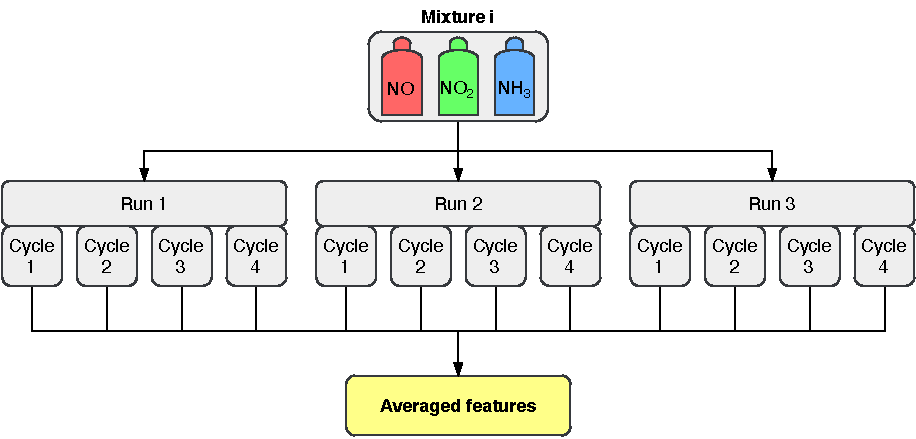
\includegraphics[width=1\textwidth]{../figures/averaging-process.pdf}
	\caption{A visualization of the feature averaging process.}
	\label{fig:averaging-process}
\end{figure}


\begin{table}
	\centering
	\caption{Sample of averaged features throughout all exposures data.}
	\label{tab:prepro-sample-unique-mixtures}
	\resizebox{\textwidth}{!}{%
		\begin{tabular}{ccp{0.8cm}p{0.8cm}p{0.8cm}p{1.8cm}p{1.8cm}p{0.3cm}p{1.6cm}p{1.6cm}p{1.6cm}p{1.6cm}p{0.3cm}p{1.6cm}p{1.6cm}}
			\toprule[0.5mm]
			Index &  UNIQUE MIXTURE &    NO &   NO2 &   NH3 &  0.05-1-slope-0 &  0.05-1-slope-1 & $\dots$&  5000.0-1-slope-239 &  0.05-1-avg-0 &  0.05-1-avg-1 &  0.05-1-avg-2 & $\dots$&  5000.0-1-avg-238 &  5000.0-1-avg-239 \\
			\midrule[0.5mm]
			0 &         0 &  5.0 &  5.0 &   5.0 &      -26.386178 &      -14.165356 &$\dots$&           -0.041897 &     28.983749 &     25.442410 &     25.383750 &$\dots$&           35.162932 &         35.152458 \\
			1 &         1 &  5.0 &  5.0 &  10.0 &      -26.294332 &      -14.421532 &$\dots$&            0.004524 &     28.538652 &     24.933269 &     24.879247 &$\dots$&           34.622460 &         34.623591 \\
			2 &         2 &  5.0 &  5.0 &  20.0 &      -25.514491 &      -15.174588 &$\dots$&           -0.010135 &     29.038925 &     25.245278 &     25.181935 &$\dots$&           35.025637 &         35.023103 \\
			3 &         3 &  5.0 &  5.0 &  40.0 &      -25.906221 &      -14.565139 &$\dots$&            0.003801 &     28.698684 &     25.057399 &     24.980686 &$\dots$&           34.575699 &         34.576649 \\
			4 &         4 &  5.0 &  5.0 &  80.0 &      -26.731849 &      -13.795072 &$\dots$&           -0.022803 &     28.738748 &     25.289980 &     25.229714 & $\dots$&          34.860040 &         34.854340 \\
			\bottomrule
			&&&&&&&&&&&&&&\\
			&&&&&&&\sbox0{\dots}\makebox[\wd0]{\vdots}&&&&&&&\\
			&&&&&&&&&&&&&&\\
			\toprule
			
			70 &        70 &  20.0 &  80.0 &   5.0 &      -26.743885 &      -13.981572 &$\dots$&            0.019546 &     28.142217 &     24.646824 &     24.596195 &$\dots$&         34.208650 &         34.213536 \\
			71 &        71 &  20.0 &  80.0 &  10.0 &      -25.832291 &      -14.650290 & $\dots$&          -0.056285 &     28.615026 &     24.952453 &     24.893228 &$\dots$&         34.511972 &         34.497900 \\
			72 &        72 &  20.0 &  80.0 &  20.0 &      -25.713207 &      -14.907192 &$\dots$&           -0.016469 &     28.432463 &     24.705665 &     24.649538& $\dots$&         34.317554 &         34.313437 \\
			73 &        73 &  20.0 &  80.0 &  40.0 &      -26.080595 &      -14.410131 &$\dots$&           -0.066238 &     28.327675 &     24.725143 &     24.685825 &$\dots$&         34.213989 &         34.197429 \\
			74 &        74 &  20.0 &  80.0 &  80.0 &      -25.091813 &      -14.220736 & $\dots$&           0.004163 &     28.611836 &     25.056652 &     24.993128 &$\dots$&         34.592507 &         34.593548 \\
			
			\bottomrule
			&&&&&&&&&&&&&&\\
			&&&&&&&\sbox0{\dots}\makebox[\wd0]{\vdots}&&&&&&&\\
			&&&&&&&&&&&&&&\\
			\toprule
			
			120 &       120 &  80.0 &  80.0 &   5.0 &      -27.073901 &      -13.562242 &$\dots$&            0.028142 &     28.548244 &     25.157684 &     25.103051 &$\dots$&         34.742313 &         34.749349 \\
			121 &       121 &  80.0 &  80.0 &  10.0 &      -26.329623 &      -14.337196 & $\dots$&          -0.012669 &     28.630183 &     25.045884 &     25.015773 & $\dots$&        34.678857 &         34.675690 \\
			122 &       122 &  80.0 &  80.0 &  20.0 &      -25.935631 &      -14.734990 & $\dots$&          -0.027690 &     28.420835 &     24.737087 &     24.687996 & $\dots$&        34.354338 &         34.347416 \\
			123 &       123 &  80.0 &  80.0 &  40.0 &      -25.821070 &      -14.855702 & $\dots$&          -0.032395 &     28.457189 &     24.743263 &     24.682929 &$\dots$&         34.327938 &         34.319839 \\
			124 &       124 &  80.0 &  80.0 &  80.0 &      -26.503363 &      -14.087625 & $\dots$&          -0.038820 &     28.615161 &     25.093255 &     25.046698 & $\dots$&        34.743829 &         34.734124 \\
			\bottomrule[0.5mm]
	\end{tabular}}
\end{table}


\begin{figure}[!htb]
	\centering
	
	\begin{subfigure}[b]{1\textwidth}
		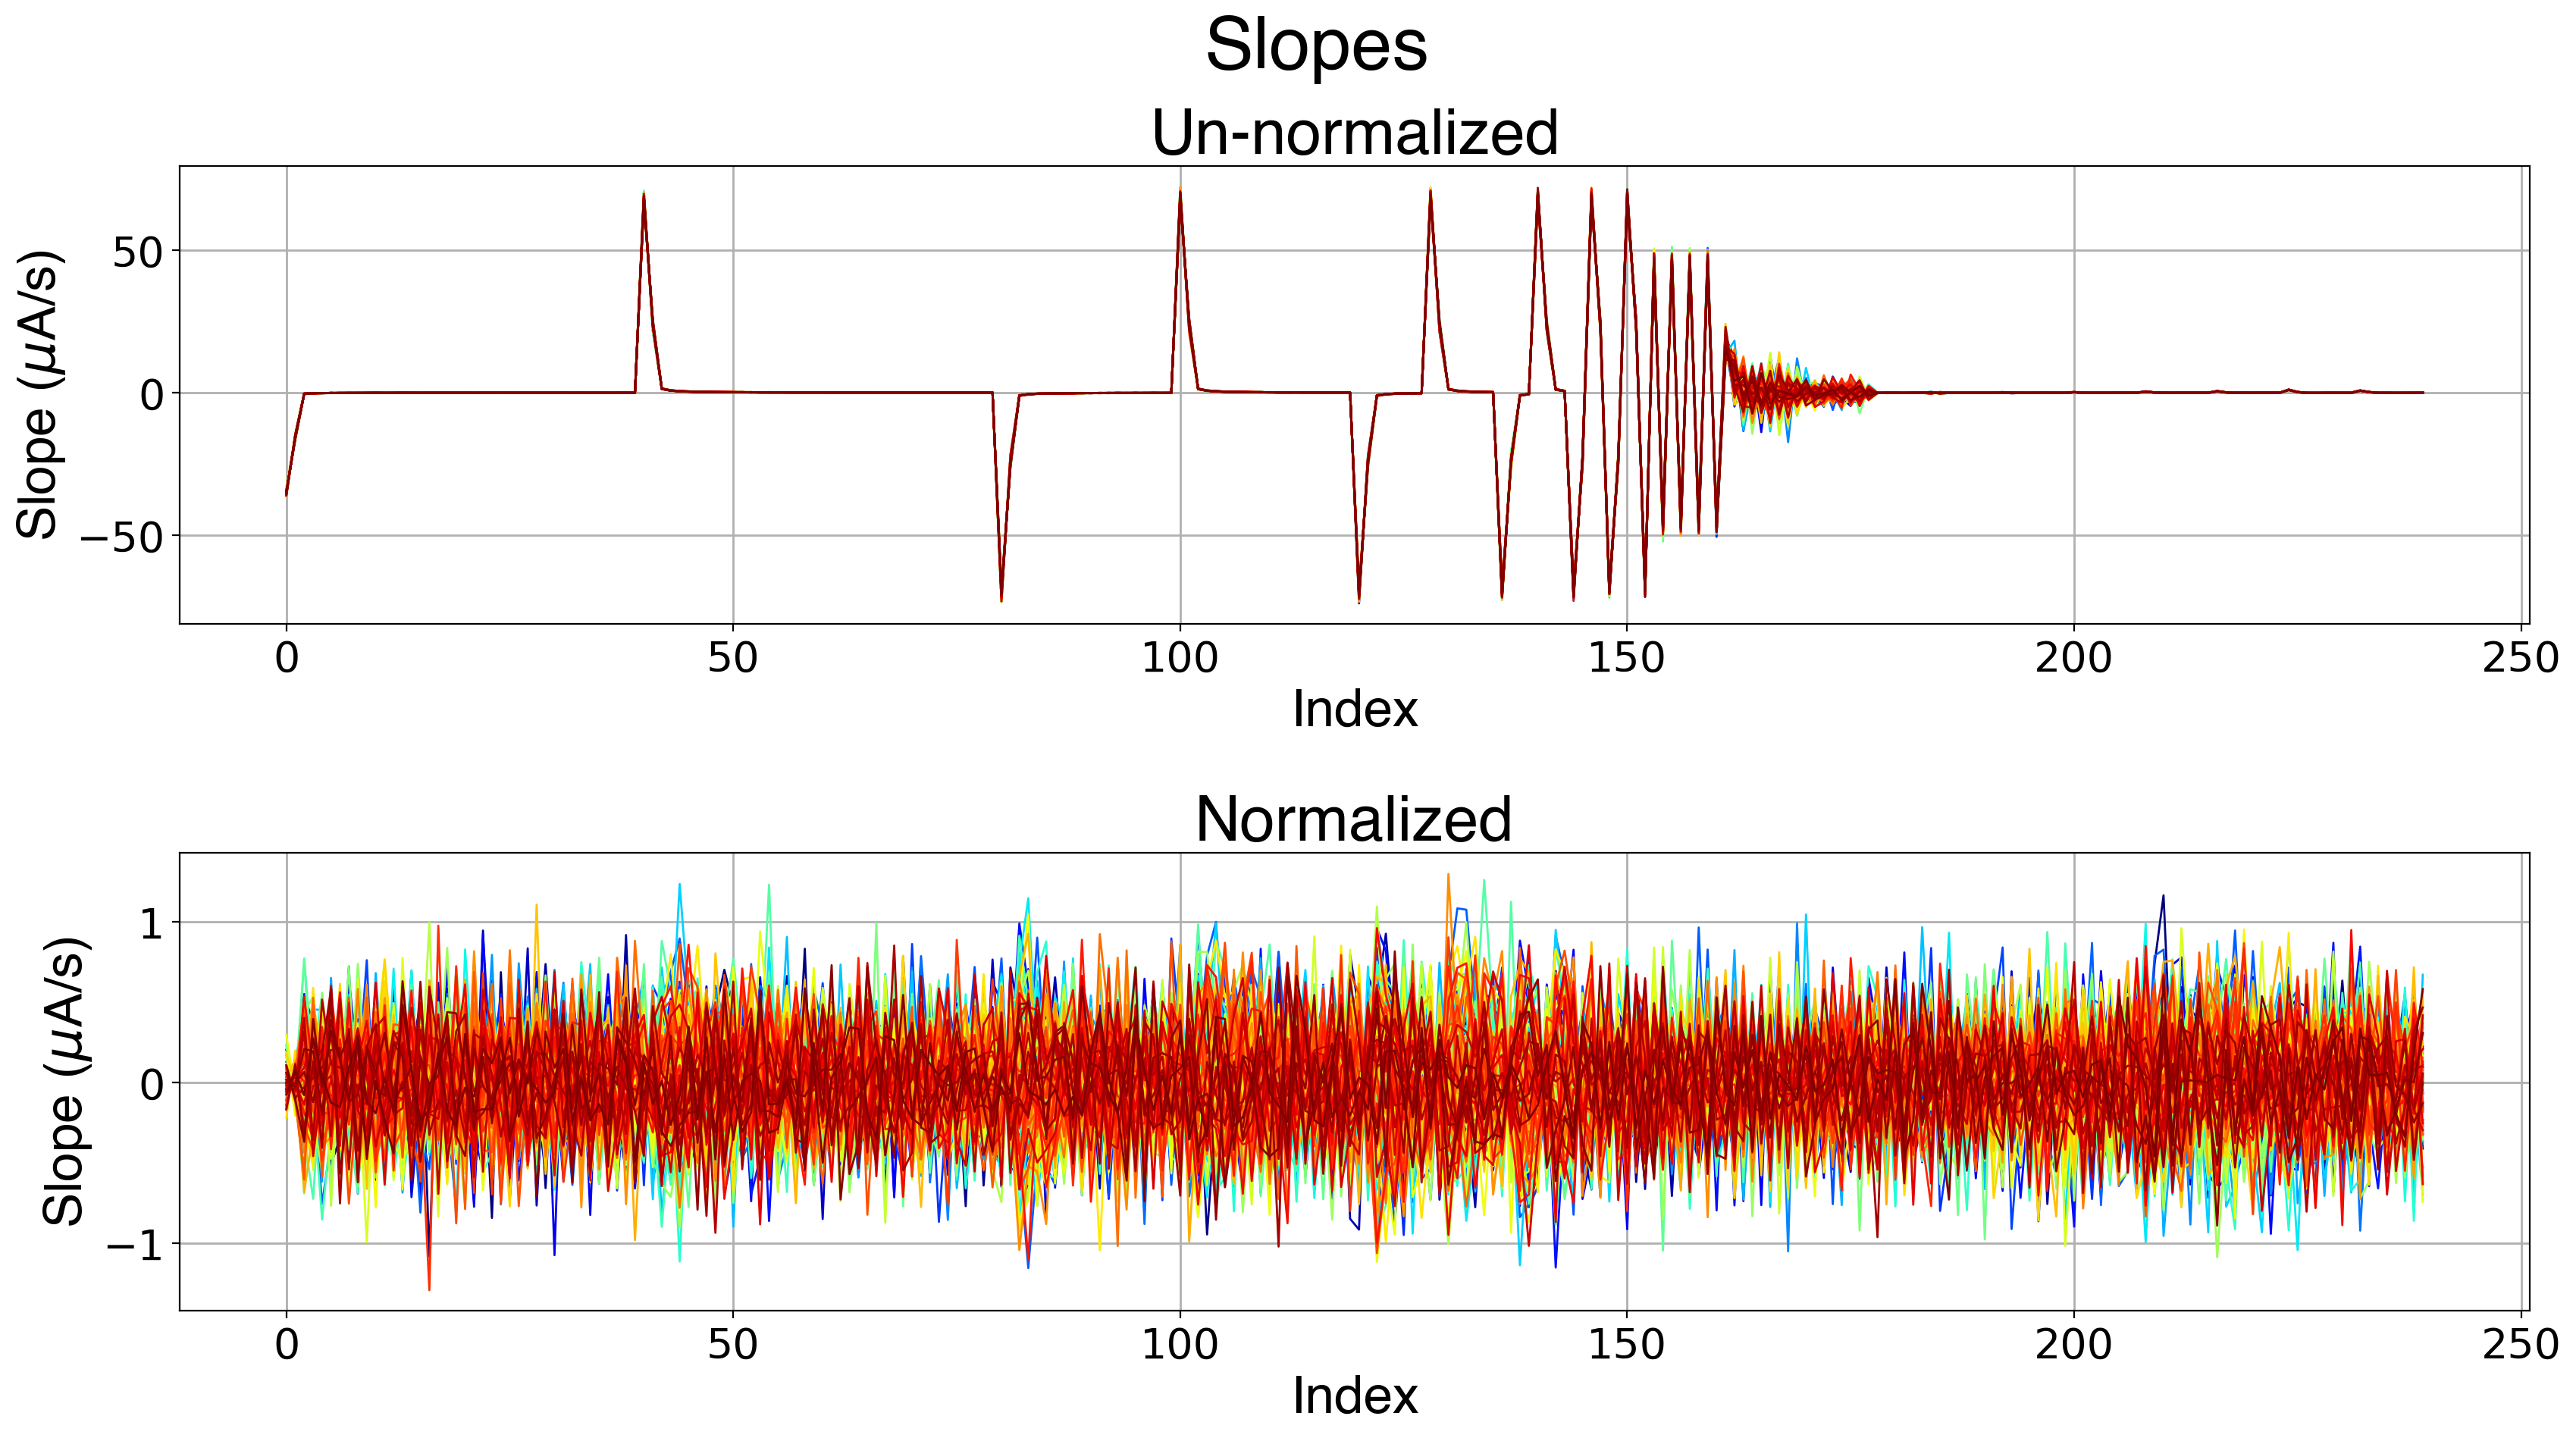
\includegraphics[width=1\linewidth]{../figures/slopes.png}
		\caption{}
		\label{fig:slopes} 
	\end{subfigure}
	
	\begin{subfigure}[b]{1\textwidth}
		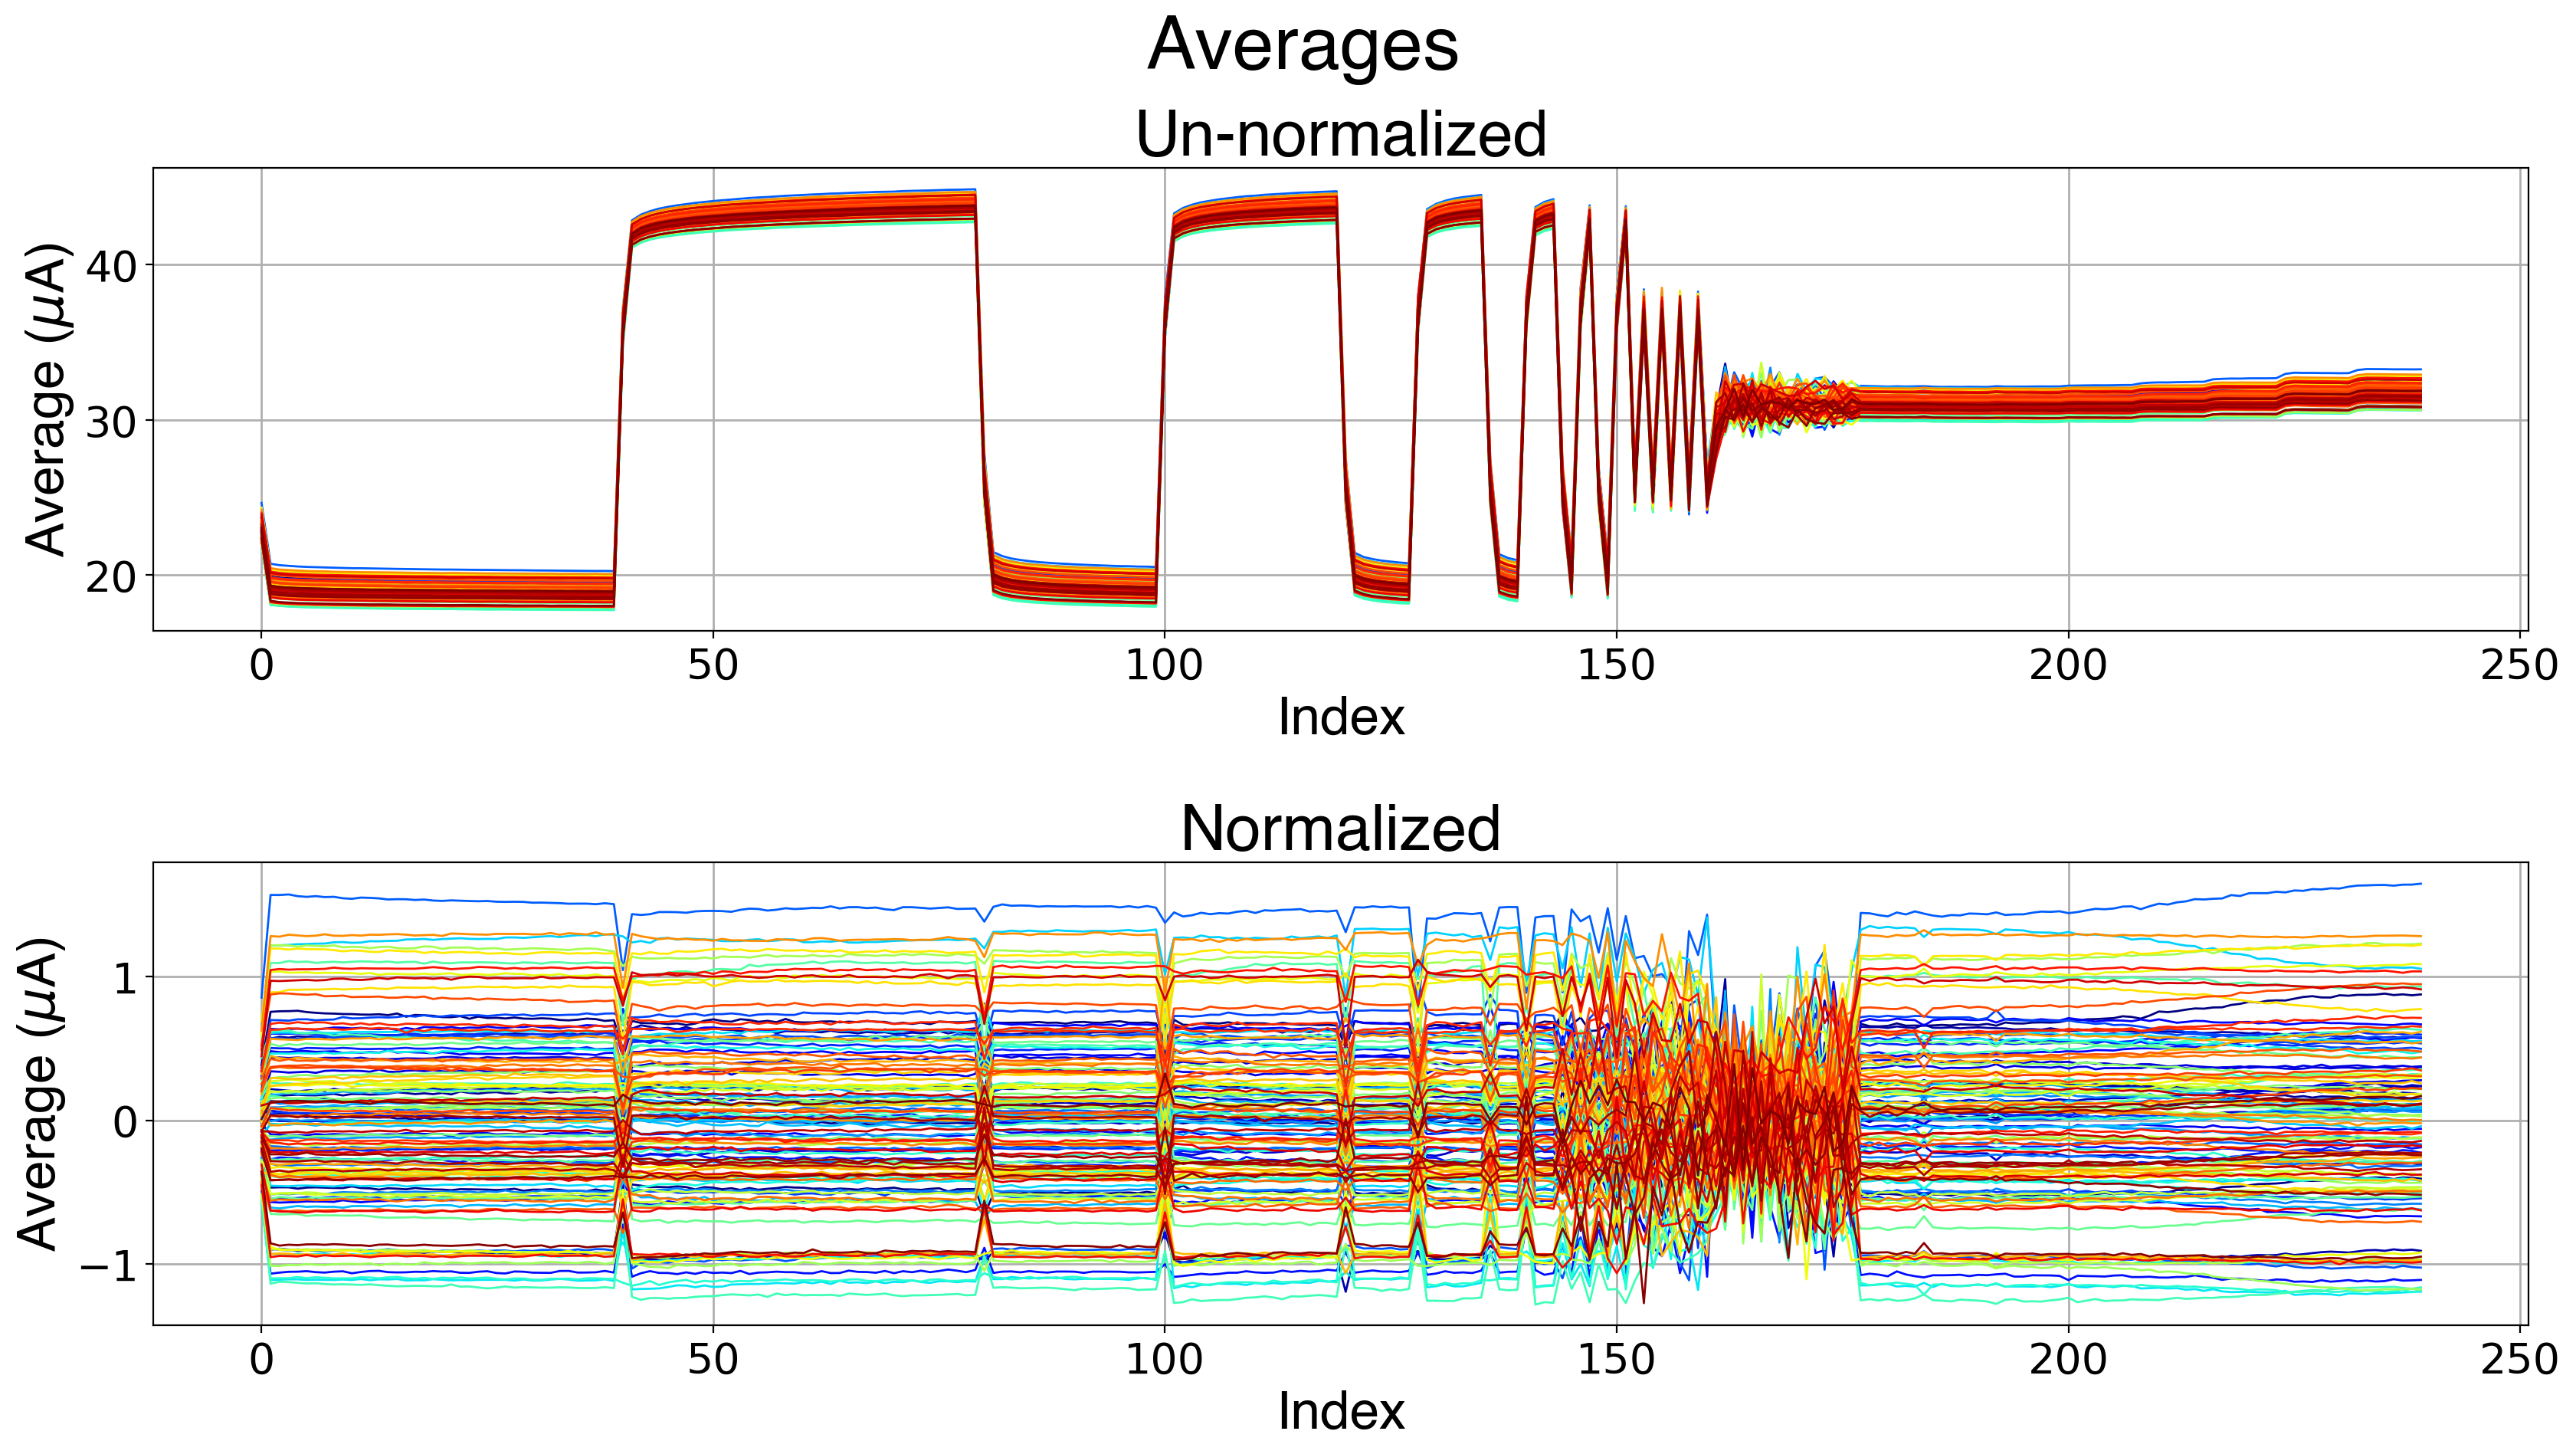
\includegraphics[width=1\linewidth]{../figures/averages.png}
		\caption{}
		\label{fig:averages}
	\end{subfigure}

	\caption{(a) Slope and (b) average features, both un-normalized and normalized.}
	\small
	In each plot, each line represents a unique gas mixture.
	\label{fig:slopes-and-averages}
\end{figure}






%%% lorem.tex --- 
%% 
%% Filename: lorem.tex
%% Description: 
%% Author: Ola Leifler
%% Maintainer: 
%% Created: Wed Nov 10 09:59:23 2010 (CET)
%% Version: $Id$
%% Version: 
%% Last-Updated: Tue Oct  4 11:58:17 2016 (+0200)
%%           By: Ola Leifler
%%     Update #: 7
%% URL: 
%% Keywords: 
%% Compatibility: 
%% 
%%%%%%%%%%%%%%%%%%%%%%%%%%%%%%%%%%%%%%%%%%%%%%%%%%%%%%%%%%%%%%%%%%%%%%
%% 
%%% Commentary: 
%% 
%% 
%% 
%%%%%%%%%%%%%%%%%%%%%%%%%%%%%%%%%%%%%%%%%%%%%%%%%%%%%%%%%%%%%%%%%%%%%%
%% 
%%% Change log:
%% 
%% 
%% RCS $Log$
%%%%%%%%%%%%%%%%%%%%%%%%%%%%%%%%%%%%%%%%%%%%%%%%%%%%%%%%%%%%%%%%%%%%%%
%% 
%%% Code:

\chapter{Theory}
\label{cha:theory}

\textcolor{blue}{Question to supervisor/examiner: Do you think this chapter goes 'deep' enough?} 

The quantification of gases based on the sensor response can be viewed as a multivariate multiple regression problem where the predictors, i.e. features derived from the sensor signal, are used to predict multiple responses, i.e. the concentrations of pertinent gases. This chapter briefly exposes the theory behind some of these models.

The models here listed were chosen as a natural progression from a statisticians point of view: starting with simple models and progressively increasing complexity as insights from the data and the problem are gathered.

\section{Ordinary Least Squares Regression}
\label{sec:linreg}

A simple, first approach would be to tackle the problem with a \acrfull{ols} regression model. As \cite{friedman2001} explains, each output  $\mathbf{Y = [y_1, y_2, ... , y_K]^\intercal} $ has its own linear model. Now, given a set of $n$ observations $\mathbf{X = [x_1, x_2, ..., x_n]^\intercal}$ and each observation having $p+1$ features, e.g. $\mathbf{x}_i = [1,x_{i1}, x_{i2}, ... x_{ip}], \; i = 1,2,...n$, the concatenation of all linear models can be written in matrix form as in Equation~\ref{eqn:ols}.

\begin{equation}
	\label{eqn:ols}
	\mathbf{Y = XB +  E}
\end{equation}

Where:
\begin{itemize}
	\item $\mathbf{B}$: [$p+1 \times K]$ matrix of regression coefficients (with the $+1$ referring to the intercept term);
	\item $\mathbf{E}$: [$N \times K]$ matrix of residuals.
\end{itemize}

The objective is then to find the coefficients $\mathbf{\hat{B}}$ which minimizes the \acrfull{rss}, which is summarized by Equation~\ref{eqn:rss} \parencite{friedman2001}:

\begin{equation}
	\label{eqn:betahat}
	\mathbf{\hat{B}^\text{OLS}} = \underset{\mathbf{B}}{\arg\min} 	\; \text{RSS}(\mathbf{B})
\end{equation}

In turn, the \acrshort{rss}, as the name suggests, is defined as the difference between real and predicted values, squared, which in matrix form is written as \parencite{friedman2001}:

\begin{equation} 
	\label{eqn:rss}
	\text{RSS}(\mathbf{B}) = \Tr [\mathbf{(Y-XB)^\intercal (Y-XB)}]
\end{equation}

Finally, solving for $\mathbf{\hat{B}}$ yields \parencite{friedman2001}:

\begin{equation}
	\label{eqn:ols_beta}
	\mathbf{\hat{B}^\text{OLS}} = \mathbf{(X^\intercal X)^{-1} X^\intercal Y}
\end{equation}

For the problem at hand, in addition to the high number of features, it is often the case that sensor data points are acquired in quick succession, which in turn leads to highly correlated features \parencite{Bastuck_2019}, which can result in high variance in a least squares model \parencite{friedman2001}. It is natural, therefore, to progress towards methods that incorporate dimensionality reduction such as \acrfull{pcr} and \acrfull{plsr} or shrinkage such as Ridge Regression.

\section{Principal Component Analysis}
\label{sec:pca}

One way to define \acrfull{pca} is to view it as a orthogonal projection of the data into a principal space of lower dimension such that the variance of this projection is maximized \parencite{bishop2006pattern}.

Just as before, consider the  collection of $n$ observations is $\mathbf{X = [x_1, x_2, ..., x_n]^\intercal}$ with covariance matrix $\mathbf{\Sigma}$. Additionally, consider a matrix $\mathbf{P = [p_1, p_2, ..., p_n]^\intercal}$ where $\mathbf{p_i}$ is a row vector of coefficients referring to the i-th linear combination \parencite{johnson2013applied}:

\begin{equation}
	\label{eqn:pca-lincomb}
	t_i=\mathbf{x_i p_i^\intercal} \;\;\;\;\;\;\;\;\;\; i = 1, 2, ..., n
\end{equation}

The variance and covariance of these new variables $t_i$ can be written as follows:

\begin{equation}
	\label{eqn:pca-var}
	\text{Var}(t_i) = \mathbf{p_i^\intercal \Sigma p_i} \;\;\;\;\;\;\;\;\;\; i = 1, 2, ..., n
\end{equation}

\begin{equation}
	\label{eqn:pca-cov}
	\text{Cov}(t_i, t_k) = \mathbf{p_i^\intercal \Sigma p_k}\;\;\;\;\;\;\;\;\;\; i,k= 1, 2, ..., n
\end{equation}

The first \acrfull{pc} is then the linear combination with maximum variance, i.e. the linear combinations that maximizes $\text{Var}(t_1)$, with the constraint that the coefficient vector $\mathbf{p_1}$ has unit length. In summary, the first \acrshort{pc} is computed as \parencite{johnson2013applied}:

\begin{equation}
	\label{eqn:pca-pc1}
	\begin{split}
		t_1 & =\mathbf{x_1 p_1^\intercal} \\
			   & \text{that maximizes Var}(\mathbf{x_1 p_1^\intercal}) \\
			   & \text{ subject to }  \mathbf{p_1^\intercal p_1} = 1
	\end{split}
\end{equation}

The second \acrshort{pc}, similarly to the first, is the linear combination with maximum variance, but with an added extra constraint: this new linear combination must be orthogonal to the previous one, i.e. they must be linearly independent:

\begin{equation}
	\label{eqn:pca-pc2}
	\begin{split}
		t_2 & =\mathbf{x_2 p_2^\intercal} \\
		& \text{that maximizes Var}(\mathbf{x_2 p_2^\intercal}) \\
		& \text{subject to }  \mathbf{p_2^\intercal p_2} = 1 \\
		& \text{and } \text{Cov}(t_1, t_2) = 0
	\end{split}
\end{equation}

The k-th \acrshort{pc} is then:

\begin{equation}
	\label{eqn:pca-pck}
	\begin{split}
		t_k & =\mathbf{x_k p_k^\intercal} \\
		& \text{that maximizes Var}(\mathbf{x_k p_k^\intercal}) \\
		& \text{subject to }  \mathbf{p_k^\intercal p_k} = 1 \\
		& \text{and } \text{Cov}(t_j, t_k) = 0 \;\;\; \text{for } k>j
	\end{split}
\end{equation}

In summary, the objective of \acrshort{pca} is find a matrix $\mathbf{P}$ such that the linear transformation

\begin{equation}
	\label{eqn:pca}
	\mathbf{T=XP^\intercal}
\end{equation}

yields new variables that are uncorrelated and arranged in decreasing order of variance.

It can be shown that these desired linear combinations can be written in terms of the eigenvalues ($\mathbf{\lambda}$) and eigenvectors ($\mathbf{e}$) of $\mathbf{\Sigma}$, the covariance matrix of $\mathbf{X}$ \parencite{johnson2013applied}. The elements of eigenvectors are called loadings, while the new features $\mathbf{T}$ are scores. In short, for the k-th \acrshort{pc}:

\begin{equation}
	\label{eqn:pca-eigen}
	\begin{split}
		t_k & =\mathbf{X_k e_k^\intercal} \\
		\text{Var}(t_k)& =  \mathbf{e_k^\intercal \Sigma e_k}=\lambda_k \\
		\text{Cov}(t_j, t_k)& = \mathbf{e_k^\intercal \Sigma e_j}= 0 \;\;\; \text{for } k\neq j
	\end{split}
\end{equation}

There are several ways of computing \acrshort{pc}s. Many of which involving finding aforementioned eigenvalues and eigenvectors. These calculations can be computationally expensive, depending on the desired number of extracted \acrshort{pc}s \parencite{bishop2006pattern}. One option is the \acrfull{nipals} algorithm, also called Power Method. It has two clear advantages: "it can handle missing data and computes the components sequentially" \parencite{dunn2021pid}.

The \acrshort{nipals} algorithm to compute the first k-th \acrshort{pc}s, $\text{PC}_i ,\;\; i =1,2,...,k$ us displayed below as Algorith~\ref{algo:pca-nipals} \parencite{dunn2021pid} \parencite{ng2013} \parencite{nipals2017}. Since it computes the loadings and scores sequentially, it is possible to stop it as early as desired. The "truncated" loadings and scores that project $\mathbf{X}$ into the principal subspace of k \acrshort{pc}s is defined in Equation~\ref{eqn:pca2} :

\begin{equation}
	\label{eqn:pca2}
	\mathbf{T_{|k}=XP_{|k}^\intercal}
\end{equation}

\begin{algorithm}[H]
	\DontPrintSemicolon
	\label{algo:pca-nipals}
	\SetAlgoLined
	\KwResult{Matrices of loadings $\mathbf{P_{|k}}$ and scores $\mathbf{T_{|k}}$  of the k-th first \acrlong{pc}s}
	Initialize $\mathbf{T_{|k}}$ and $\mathbf{P_{|k}}$\;
	i = 1\;
	$\mathbf{X_1 \coloneqq X}$\;
	
	\While{$i < k$ }{\Repeat{$\mathbf{t_i}$ converges}{
			Choose $\mathbf{t_i}$ as any column of $\mathbf{X_i}$\;
			Compute loadings $\mathbf{p_i = (t_i^\intercal t_i)}^{-1} \mathbf{t_i^\intercal X_i}$\;
			Scale $\mathbf{p_i = \frac{p_i}{\sqrt{p_i^\intercal p_i}}}$\;
			Compute scores $\mathbf{t_i = (p_i^\intercal p_i)}^{-1}\mathbf{p_i^\intercal X_i}$\;
		}
	Append $\mathbf{t_i}$ to $\mathbf{T_{|k}}$\;
	Append $\mathbf{p_i}$ to $\mathbf{P_{|k}}$\;
	Deflate: $\mathbf{X_{i+1} = X_i - t_i p_i^\intercal}$\;
	$i \mathrel{+}= 1$\;
	}
	\KwRet{$\mathbf{T_{|k}, P_{|k}}$}	
	
	\caption{\acrfull{nipals} for \acrshort{pca}}
\end{algorithm}

In other words:

\begin{itemize}
	\item Line 1: Initilize the algorithm taking into account all data $\mathbf{X}$;
	
	\item Line 6: Arbitrarily choose a column of $\mathbf{X}$ as the scores vector $\mathbf{t_i}$;
	
	\item Line 7: Compute the i-th loadings vector $\mathbf{p_i}$ by regressing every column of $\mathbf{X}$ via \acrshort{ols} onto the scores $\mathbf{t_i}$;
	
	\item Line 8: Scale the loadings vector $\mathbf{p_i}$ to have unit length;
	
	\item Line 9: Compute the i-th scores vector $\mathbf{t_i}$ by regressing every column of $\mathbf{X}$ via \acrshort{ols} onto the loadings $\mathbf{p_i}$;
	
	\item Line 10: Repeat until change in $\mathbf{t_i}$ between iterations is small enough;
	
	\item Lines 11 and 12: Once convergence is achieved, scores $\mathbf{t_i}$ and loadings $\mathbf{p_i}$ are stored as the i-th column of matrices $\mathbf{T}$ and $\mathbf{P}$ of Equation~\ref{eqn:pca}, respectively;
	
	\item Line 13: Remove the variability explained by $\mathbf{t_i}$ and $\mathbf{p_i}$ from $\mathbf{X}$. A procedure called deflation.
\end{itemize}

\section{Principal Component Regression}
\label{sec:pcr}

With the inner workings of \acrshort{pca} explained in the previous section, \acrshort{pcr} can be simply reduced to a Least Squares regression on the first k-th \acrshort{pc}s, i.e. performing linear regression on $\mathbf{T_{|k}}$ instead of $\mathbf{X}$:
	
	\begin{equation}
		\label{eqn:pcr}
		\mathbf{Y = T_{|k} B + E}
	\end{equation}

And the regression coefficients are found analogously to Equation~\ref{eqn:ols_beta}:

\begin{equation}
	\label{eqn:beta-pcr}
	\mathbf{\hat{B}^{\text{PCR}} = (T_{|k}^\intercal T_{|k})^{-1}T_{|k}^\intercal Y}
\end{equation}

Although useful, \acrshort{pcr} has a potential flaw: while the new found projection of $\mathbf{X}$ is guaranteed to best explain the variance of predictors, this cannot be said about the responses $\mathbf{Y}$ \parencite{james2013introduction}. \acrshort{plsr}, on the other hand, solves this issue by supervising the identification of \acrshort{pc}s \parencite{james2013introduction}.
	
\section{Partial Least Squares Regression}
\label{sec:plsr}

\acrshort{plsr}, much like \acrshort{pcr}, also aims to reduce dimensionality via linear combinations of the inputs. This technique, however, also takes into account the response variables $\mathbf{Y}$. One key advantage of \acrshort{plsr} is that it seeks axes with most variance (like \acrshort{pcr}) and high correlation with response variables \parencite{friedman2001}.

The main idea can be described as  finding  linear combinations  for the data matrix design matrix $\mathbf{X}$ and response matrix $\mathbf{Y}$ as follows \parencite{ng2013}, similarly to what was done in Section~\ref{sec:pca}.

\begin{equation}
	\label{eqn:x-decomp}
	\mathbf{W=XL^\intercal}
\end{equation}

\begin{equation}
	\label{eqn:y-decomp}
	\mathbf{U = YQ^\intercal}
\end{equation}

Instead of simply running \acrshort{nipals} on $\mathbf{X}$ and $\mathbf{Y}$ separately. \acrshort{plsr} uses information from $\mathbf{Y}$ to decompose $\mathbf{X}$ and \textit{vice-versa} \parencite{ng2013}. Algorithm~\ref{algo:pls-nipals} is an adaptation of Algorithm~\ref{algo:pca-nipals} to incorporate this intended behavior.

\begin{algorithm}[H]
	\DontPrintSemicolon
	\label{algo:pls-nipals}
	\SetAlgoLined
	\KwResult{Matrices of loadings $\mathbf{L_{|k}, Q_{|k}}$ and scores $\mathbf{W_{|k}, U_{|k}}$  of the k-th first \acrlong{pls} directions}
	Initialize $\mathbf{L_{|k}, Q_{|k}}$ and $\mathbf{W_{|k}, U_{|k}}$\;
	i = 1\;
	$\mathbf{X_1 \coloneqq X}$\;
	$\mathbf{Y_1 \coloneqq Y}$\;
	
	\While{$i < k$ }{\Repeat{$\mathbf{u_i}$ converges}{
			Choose $\mathbf{u_i}$ as any column of $\mathbf{Y_i}$\;
			
			Compute loadings of $\mathbf{X_i}$ based on score of $\mathbf{Y_i}$: $\mathbf{\ell_i = (u_i^\intercal u_i)}^{-1} \mathbf{u_i^\intercal X_i}$\;
			
			Scale $\mathbf{\ell_i = \frac{\ell_i}{\sqrt{\ell_i^\intercal \ell_i}}}$\;
			
			Compute score of $\mathbf{X_i}$: $\mathbf{w_i = (\ell_i^\intercal \ell_i)}^{-1}\mathbf{\ell_i^\intercal X_i}$\;
			
			Compute loadings of $\mathbf{Y_i}$ based on score of $\mathbf{X_i}$: $\mathbf{q_i = (w_i^\intercal w_i)}^{-1} \mathbf{w_i^\intercal Y_i}$\;
			
			Scale $\mathbf{q_i = \frac{q_i}{\sqrt{q_i^\intercal q_i}}}$\;
			
			Compute score of $\mathbf{Y_i}$: $\mathbf{u_i = (q_i^\intercal q_i)}^{-1}\mathbf{q_i^\intercal Y_i}$\;
		}
		Append $\mathbf{w_i}$ to $\mathbf{W_{|k}}$\;
		Append $\mathbf{\ell_i}$ to $\mathbf{L_{|k}}$\;
		Append $\mathbf{u_i}$ to $\mathbf{U_{|k}}$\;
		Append $\mathbf{q_i}$ to $\mathbf{Q_{|k}}$\;
		Deflate $\mathbf{X_i}$: $\mathbf{X_{i+1} = X_i - w_i \ell_i^\intercal}$ \;
		Deflate $\mathbf{Y_i}$:	$\mathbf{Y_{i+1} = Y_i - u_i q_i^\intercal}$ \;
		$i \mathrel{+}= 1$\;
	}
	\KwRet{$\mathbf{W_{|k}, L_{|k}, U_{|k}, Q_{|k}}$}	
	\caption{\acrshort{nipals} for \acrfull{plsr}}
\end{algorithm}

In summary, highlighting the most important parts: 

\begin{itemize}
	\item  Line 7: Arbitrarily choose a column of $\mathbf{Y_i}$ as the initial response score vector $\mathbf{u_i}$;
	
	\item Line 8: Compute the i-th loadings vector $\mathbf{w_i}$  of $\mathbf{X}$  by regressing every column of $\mathbf{X}$ via \acrshort{ols} onto scores vector of $\mathbf{Y}$, $\mathbf{u_i}$;
	
	\item Line 9: Scale the data loadings vector $\mathbf{w_i}$ to have unit length;
	
	\item Line 10: Compute the i-th data scores vector $\mathbf{w_i}$ by regressing every column of $\mathbf{X_i}$ via \acrshort{ols} onto the column $\mathbf{\ell_i}$;
	
	\item 	Line 11: Compute the i-th loadings vector $\mathbf{q_i}$  of $\mathbf{Y_i}$  by regressing every column of $\mathbf{Y}$ via \acrshort{ols} onto scores vector of $\mathbf{X}$, $\mathbf{w_i}$;
	
	\item Line 12: Scale the response loadings vector $\mathbf{q_i}$ to have unit length;
	
	\item Line 13: Compute the i-th response scores vector $\mathbf{u_i}$ by regressing every column of $\mathbf{Y_i}$ via \acrshort{ols} onto the column $\mathbf{q_i}$;
	
	\item Line 14: Repeat until change in $\mathbf{u_i}$ between iterations is small enough;

	\item Lines 15 and 16: Once convergence is achieved, $\mathbf{w_i}$ and $\mathbf{\ell_i}$ are stored as the i-th column of matrices $\mathbf{W}$ and $\mathbf{L}$ of Equation~\ref{eqn:x-decomp};
	
	\item Lines 17 and 18: Once convergence is achieved, $\mathbf{u_i}$ and $\mathbf{q_i}$ are stored as the i-th column of matrices $\mathbf{U}$ and $\mathbf{Q}$ of Equation~\ref{eqn:y-decomp};
	
	\item Lines 19 and 20: Remove the variability explained by $\mathbf{w_i, \ell_i}$ and $\mathbf{u_i, q_i}$ from $\mathbf{X_i}$ and $\mathbf{Y_i}$, respectively;
	
\end{itemize}

After finding the $k$ partial least squares directions from Algorithm~\ref{algo:pls-nipals} above, the problem, as in Section~\ref{sec:pcr}, reduces to performing Least Squares Regression using the newfound transformations.

	\begin{equation}
	\label{eqn:plsr}
	\mathbf{Y = W_{|k} B + E}
\end{equation}

Which in turn, analogously to Equations~\ref{eqn:ols_beta} and \ref{eqn:beta-pcr} yields the coefficients:

\begin{equation}
	\label{eqn:beta-plsr}
	\mathbf{\hat{B}^{\text{PLSR}} = (W_{|k}^\intercal W_{|k})^{-1}W_{|k}^\intercal Y}
\end{equation}

\section{Ridge Regression}
\label{sec:ridge}

Ridge regression is also a viable alternative to reduce the problem of highly correlated features \parencite{friedman2001}. Instead of fitting a least squares model on a subset of predictors or a transformation of them, Ridge allows the use of all features with a continuous shrinkage of its coefficients, which results in less variance \parencite{friedman2001}.



For the multi-output case, there are two options: use the same penalization parameter $\lambda$ for all variables $\mathbf{Y = [y_1, y_2, ... , y_K]^\intercal}$ or apply different parameters $\mathbf{\boldsymbol{\lambda} = [\lambda_1, \lambda_2, ... , \lambda_K]^\intercal}$. In this work, the latter is preferred over the former, as it allows a more fine tuned control of the regression models for each studied gas.

Analogous to Section~\ref{sec:linreg}, the goal is to minimize the \acrshort{rss}, but now with the penalization term taken into account. Equation~\ref{eqn:rss-ridge} below shows this objective function in matrix form.

\begin{equation} 
	\label{eqn:rss-ridge}
	\text{RSS}^{\text{Ridge}}(\mathbf{B, \boldsymbol{\lambda} }) = \Tr [\mathbf{(Y-XB)^\intercal (Y-XB)}] + \Tr[\mathbf{B^\intercal B + \boldsymbol{\lambda} I}]
\end{equation}

\begin{equation}
	\label{eqn:betahat-ridge}
	\mathbf{\hat{B}^\text{Ridge}} = \underset{\mathbf{B}}{\arg\min} 	\; \text{RSS}^{\text{Ridge}}(\mathbf{B})
\end{equation}	

The coefficients that minimize the \acrshort{rss} is shown in Equation~\ref{eqn:eqn:betahat-ridge2} below.

\begin{equation}
	\label{eqn:eqn:betahat-ridge2}
	\mathbf{\hat{B}^\text{Ridge}} = \mathbf{(X^\intercal X + \boldsymbol{\lambda}  I )^{-1} X^\intercal Y}
\end{equation}

The choice of hyper-parameters $\boldsymbol{\lambda} \geq 0$ controls how much shrinkage is applied to the coefficients: larger $\boldsymbol{\lambda}$ implies more penalization to complex models. Although the coefficients are shrunk towards zero, they never reach zero, which makes Ridge regularization unsuitable for feature selection \parencite{friedman2001}.

This 

\section{Cross Validation}
\label{sec:crossval}

\section{Bootstrapping}
\label{sec:hypot}


With the theoretical background laid out, this work proceeds to present the data, its acquisition and its features.

%%%%%%%%%%%%%%%%%%%%%%%%%%%%%%%%%%%%%%%%%%%%%%%%%%%%%%%%%%%%%%%%%%%%%%
%%% lorem.tex ends here

%%% Local Variables: 
%%% mode: latex
%%% TeX-master: "demothesis"
%%% End: 

\chapter{Methods}
\label{cha:methods}

This work's main question is: given sensor responses, how one can quantify the gases that produced them? Multivariate regression techniques have been shown to be successful, namely \acrfull{plsr} has been used in chemometrics extensively and it has been proven to be good at this task \parencite{Bastuck_2019} \parencite{wold2011}.

For example, \textcite{BUR2015225} uses \acrshort{tco} of \acrshort{sicfet} sensors alongside \acrshort{plsr} to quantify naphthalene sufficiently enough to monitor its concentration for indoor air quality monitoring. Additionally, \textcite{BASTUCK2016263} shows that, also using \acrshort{tco}, \acrshort{plsr} can  quantify ethanol and naphthalene mixtures down to the \acrfull{ppb} level.

All code was done in Python, namely in Jupyter notebooks, both for it's simplicity and for its easiness in code and data exploration. In general, the use of Python's library Scikit-Learn and its \texttt{pipeline} class alongside linear models made analysis straightforward. Additionally, Scikit-Learn's \texttt{GridSearchCV} allowed for a faster evaluation of different hyperparameters such as the number of components and shrinkage factors. 

Throughout all methods, training and test sets were split using Python's \texttt{train\_test\_split} function. 80\% of observations were assigned to the training set and the remaining 20\% to the test set. A fixed random seed of 42 was set to ensure reproducibility of results. All cross-validation evaluations were done with 5 folds.

Before any model implementation, however, the data needed to be pre-processed as described in Section~\ref{sec:preprocessing}. This was done by "transposing" the row-based, per sample  measurements into column-based, per exposure features. This reduces the number of row significantly: from 360.000 to 1500. The features were named according to Figure~\ref{fig:feat-naming}.

The evaluation and comparison of different models was made via the actual vs. predicted  plot. In it, it is possible to qualitatively see how good the predictions are. Additionally, fit metrics such as $\text{R}^2$ and \acrshort{rmse} are shown as a quantitative means of comparison.

This methodology was carried out using data from both sensors: 1 and 2. Moreover, two variations of the data from these sensors were used: first using 1500 exposures and all 480 features. The second variation was done by averaging all exposures into unique mixtures as described in Figure~\ref{fig:averaging-process} and only using average features, as described in Chapter~\ref{cha:data}.

Although all models are linear, attempts at introducing polynomial regression terms were made. However, results from these attempts were similar to the linear fit. On top of that, the addition of polynomial degrees in cross-validation grid search made computations extremely slow. Given the computational and time constraints at hand, this approach was discarded.

For further details regarding coding and implementation, the reader is referred to this work's \href{https://github.com/cosmourao/thesis}{\textcolor{blue}{repository}}, where all notebooks can be found.

\section{\acrlong{ols}}
\label{sec:met-ols}

Here treated as a baseline, \acrshort{ols} is fit using all 480 features and evaluated using the test set. 

\section{\acrlong{pcr}}
\label{sec:met-pcr}

First, a \acrshort{pca} with two \acrshort{pc}s was performed. With that, cumulative variance and score plots were made in an attempt of better visualizing and understanding the data.

Following that, a linear regression on the \acrshort{pc}s was made. The number of components was set to be between 1 and 200, and the ideal number of components was chosen via cross-validation with \acrshort{rmse} as the scoring function. Just as before, the ideal model was evaluated in a held-out test set, and an actual-vs-predicted plot was constructed.

\section{\acrlong{plsr}}
\label{sec:met-plsr}

Here, a similar procedure to Section~\ref{sec:met-pcr} was conducted. Initially, two \acrshort{pls} components were extracted, and some informative plots were made: cumulative explained variance and score plots in an attempt to better visualize the data. Here, once more, the grid of the number of \acrshort{pls} components was set between 1 and 200. The regression model was trained with the ideal number of components given by \acrshort{cv} and later evaluated in the held-out test set.

\section{Ridge Regression}
\label{sec:met-ridge}

For the shrinkage factor $\phi$, a logarithmic grid of 1000 values of  $\phi$, ranging from $10^{-10} $ to $10^4$ was set. This deliberate choice of  unusually high values of $\phi$ is further explained in Chapter~\ref{cha:discussion}. Regardless of that, \acrshort{cv} was used to find the best fit and that was evaluated in the held-out test set.
%%% lorem.tex --- 
%% 
%% Filename: lorem.tex
%% Description: 
%% Author: Ola Leifler
%% Maintainer: 
%% Created: Wed Nov 10 09:59:23 2010 (CET)
%% Version: $Id$
%% Version: 
%% Last-Updated: Wed Nov 10 09:59:47 2010 (CET)
%%           By: Ola Leifler
%%     Update #: 2
%% URL: 
%% Keywords: 
%% Compatibility: 
%% 
%%%%%%%%%%%%%%%%%%%%%%%%%%%%%%%%%%%%%%%%%%%%%%%%%%%%%%%%%%%%%%%%%%%%%%
%% 
%%% Commentary: 
%% 
%% 
%% 
%%%%%%%%%%%%%%%%%%%%%%%%%%%%%%%%%%%%%%%%%%%%%%%%%%%%%%%%%%%%%%%%%%%%%%
%% 
%%% Change log:
%% 
%% 
%% RCS $Log$
%%%%%%%%%%%%%%%%%%%%%%%%%%%%%%%%%%%%%%%%%%%%%%%%%%%%%%%%%%%%%%%%%%%%%%
%% 
%%% Code:

\chapter{Results}
\label{cha:results}


%%%%%%%%%%%%%%%%%%%%%%%%%%%%%%%%%%%%%%%%%%%%%%%%%%%%%%%%%%%%%%%%%%%%%%
%%% lorem.tex ends here

%%% Local Variables: 
%%% mode: latex
%%% TeX-master: "demothesis"
%%% End: 

\chapter{Discussion}
\label{cha:discussion}

This chapter is dedicated to explaining the results obtained in the previous sections and relating them to statistical theory. The main objective here is to explain why the results are not satisfactory for gas concentration predictions.

\section{Results}
\label{sec:discussion-results}

From the results shown in Chapter~\ref{cha:results}, it is clear that all models fail in predicting gas concentrations. As a first visual assessment, it can be seen from Figures~\ref{fig:slopes} and \ref{fig:averages} that there seems to be no clear order of response variables, i.e. simultaneous gas concentrations.

 Slope features, for example, are approximately zero throughout the cycle, with the exception of some particular measurements, as seen in Figure~\ref{fig:slopes}. Even then, visual inspection indicates that this feature is not informative of gas concentrations. For this reason, the second part of the analysis was done without these features.
 
 Average features, on the other hand, seem to have some separation and indicate that gas concentrations might be explained by it. Nonetheless, it is not possible to order in any clear way. For example, mixtures with high concentrations of NO have average features that vary widely, and it does not seem to follow any particular linear order of ammonia or \nox concentration levels. Further attempts at ordering the data can be found in Appendix~\ref{app:B}. 
 
\acrlong{ols} was expected to perform poorly due to the high correlation of average features evidenced in Figure~\ref{fig:cor-mat}. Indeed, the results fail to predict gas concentrations at a reasonable level, as seen in Figure~\ref{fig:ols-exposures}. Looking at the actual vs. predicted plot, it can be seen that the predictions are centered at the mean of concentrations (31 ppm) and have high variance, indicated by the wide range of prediction in all concentration levels.

\acrshort{pca} with two components confirmed previous suspicions: there is no clear separation of gas concentrations for any of the gases. Although Figure~\ref{fig:pca-exp-var-both} shows that 80\% of the variance can be explained by approximately 80 components, cross-validation indicate that only one \acrshort{pc} yields minimal error. Predictions in Figure~\ref{fig:pcr-both} are poor but have significantly less variance around the concentration mean than \acrshort{ols}. This is expected from this method, as the extraction of \acrshort{pc}s is tightly related to the explained variability of the predictors, selecting linear combinations ordered by "importance" to the result.

\acrshort{plsr}, a method that has been shown to work in this type of problem, also performed poorly. Once again, there is no clear separation of concentration levels as shown in Figure~\ref{fig:pls-both}, and \acrshort{cv} shows that only one component, again, yields minimal \acrshort{rmse}. Prediction results in Figure~\ref{fig:plsr-actual-vs-pred-both} is very similar to predictions from \acrshort{pcr}: centered around the mean with lower variance than \acrshort{ols}. The similarity in these results can be explained by the poorness of fit: both models perform "better" in the test set when under-fitting the data, i.e. the models failed to capture the relationship between input and output.

The final proposed model, Ridge regression, also fails completely in prediction, but brings meaningful insights for analysis. The \acrshort{cv} plot for the shrinkage factor $\lambda$ shows a curious behavior: with low values of $\lambda$, regression seems to fit training data well, with a relatively low \acrshort{rmse} of approximately 23. However, this is not the case for the test set. From the plot, extremely high values of regularization yield the lowest \acrshort{rmse} in the test set, around 27. From Equations~\ref{eqn:ridgebetahat2}, \ref{eqn:ridge-betazero} and \ref{eqn:ridge-yhat}, it can be seen that for high $\lambda$, the regression converges to a model that only predicts the mean (in this case, 31 ppm). A virtually "infinite" regularization would achieve the best predictions in this case.

\section{Future work}
\label{sec:discussion-method}

In hindsight, the results indicate that the selection of linear models was ill-advised. Although \acrshort{plsr} seems to work well for problems using \acrshort{tco}, this is not the case for frequency modulation with \nox and ammonia. For future work, non-parametric models are recommended. Perhaps their high flexibility and  lack of assumptions about data could be of aid in achieving better prediction metrics.

Additionally, the frequency cycle itself could be changed. Most notably, instead of a square wave signal, a triangular wave could be more desired, as it would imply in less "stable" sections of the sensor response, possibly yielding more meaningful features, specially slopes.

Another possible point of exploration is the measurement window size. A too-narrow window in combination with a square wave signal might concentrate information on a few observations per frequency only, e.g. the binary-like behavior of the slope features. In this sense, higher lower sampling frequencies could aid in extracting more meaningful features.

\section{The work in a wider context}
\label{sec:work-wider-context}

From a statisticians point of view, it is always a misfortune when analysis' results are not "good" in the sense of high accuracy or low prediction error. These arbitrarily "bad" results, however, bring more insight to the problem, and knowing what does not work might be as valuable as knowing what works.

The quantification of \nox and Ammonia, as shown in Chapter~\ref{cha:introduction}, is of paramount importance in the current world, where combustion processes are still commonplace. Although the advent of ever-improving electric vehicles is a silver lining regarding gas emissions and combustion processes, some industrial processes cannot avoid it. 

%%%%%%%%%%%%%%%%%%%%%%%%%%%%%%%%%%%%%%%%%%%%%%%%%%%%%%%%%%%%%%%%%%%%%%
%%% lorem.tex ends here

%%% Local Variables: 
%%% mode: latex
%%% TeX-master: "demothesis"
%%% End: 

%%% lorem.tex --- 
%% 
%% Filename: lorem.tex
%% Description: 
%% Author: Ola Leifler
%% Maintainer: 
%% Created: Wed Nov 10 09:59:23 2010 (CET)
%% Version: $Id$
%% Version: 
%% Last-Updated: Wed Nov 10 09:59:47 2010 (CET)
%%           By: Ola Leifler
%%     Update #: 2
%% URL: 
%% Keywords: 
%% Compatibility: 
%% 
%%%%%%%%%%%%%%%%%%%%%%%%%%%%%%%%%%%%%%%%%%%%%%%%%%%%%%%%%%%%%%%%%%%%%%
%% 
%%% Commentary: 
%% 
%% 
%% 
%%%%%%%%%%%%%%%%%%%%%%%%%%%%%%%%%%%%%%%%%%%%%%%%%%%%%%%%%%%%%%%%%%%%%%
%% 
%%% Change log:
%% 
%% 
%% RCS $Log$
%%%%%%%%%%%%%%%%%%%%%%%%%%%%%%%%%%%%%%%%%%%%%%%%%%%%%%%%%%%%%%%%%%%%%%
%% 
%%% Code:

\chapter{Conclusion}
\label{cha:conclusion}

Given previous discussions and analysis, the answer to the research question "Can frequency modulation be used to simultaneously quantify \nox and Ammonia concentrations?" seems to be: "perhaps not". Although poor predictions, the methods used here are far from exhausting the several other, possibly more flexible, models in the statisticians' toolbox. Moreover, experiments using different frequency modulations (e.g. triangular waves instead of square) and/or different sensor calibrations and/or different temperatures could be further investigated to answer this question conclusively.

As for the second question, "Does the quality of fit varies over different prediction models?", the correct answer would be "no". All models failed to predict gas concentrations in every concentration, and \acrshort{cv} results indicate that an under fitted, predict-the-mean model seems to work best in every situation, indicating that the models were not suitable for the regression analysis, as indicated by the $\text{R}^2$ tending to zero in most models.

The author finds comfort in perhaps pointing future work towards better methods and possibly better quantification of these gases in hopes of addressing the problem more efficiently than current practices. In this sense, this thesis work is considered successful.


\printbibliography


\appendix


\chapter{Data acquisition time stamps}
\label{app:A}
	
	\begin{table}[!htb]
		
		\centering
		\caption{Data acquisition timestamps.}
		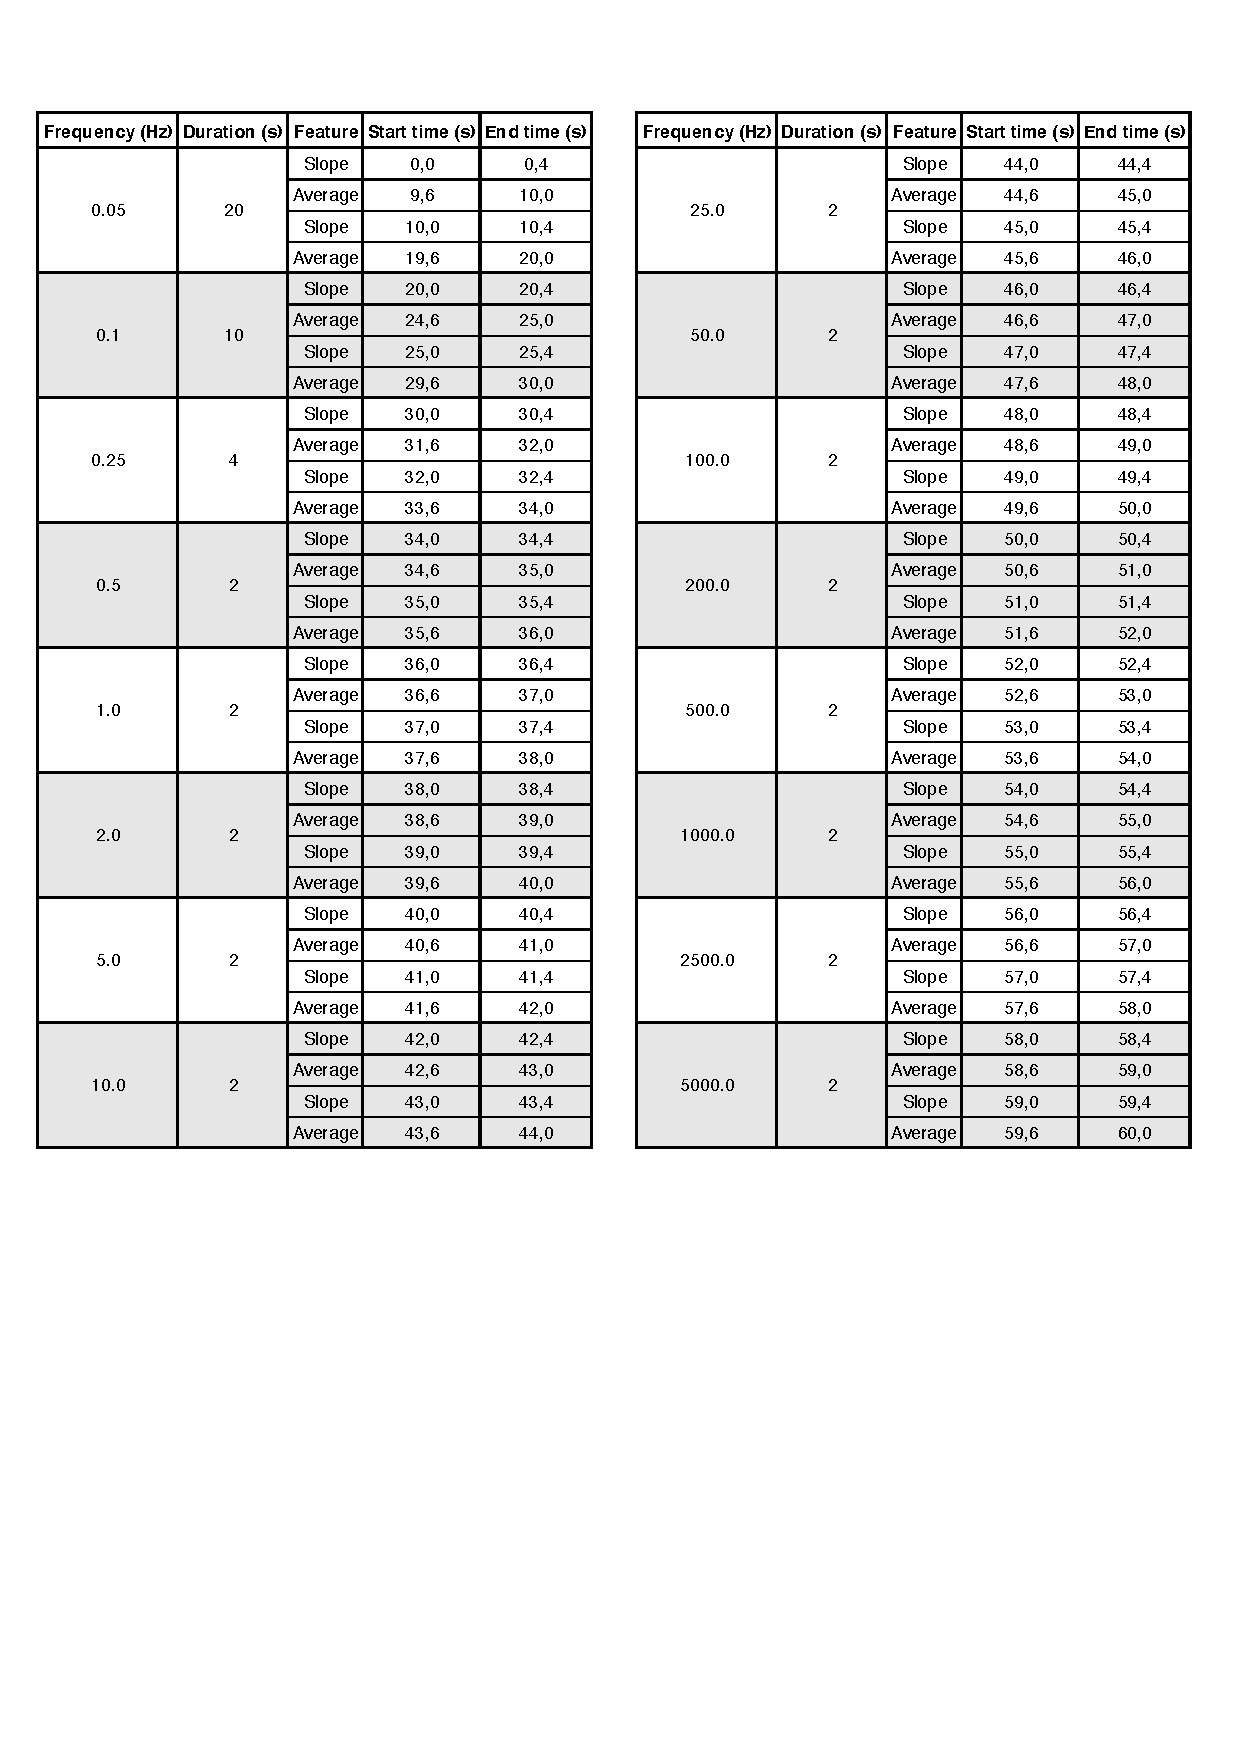
\includegraphics[width=0.99\textwidth]{../figures/timestamps.pdf}
		\label{fig:timestamps}
		
	\end{table}
%

\end{document}

%%%%%%%%%%%%%%%%%%%%%%%%%%%%%%%%%%%%%%%%%%%%%%%%%%%%%%%%%%%%%%%%%%%%%%
%%% demothesis.tex ends here

